% -*- mode: noweb; noweb-default-code-mode: R-mode; -*-
\documentclass[nojss]{jss}
\include{graphicx}
%%%%%%%%%%%%%%%%%%%%%%%%%%%%%%%%%%%%%%%%%%%%%%%%%%%%%%%%%%%%%%%
%% declarations for jss.cls - journal of statistical software
%%%%%%%%%%%%%%%%%%%%%%%%%%%%%%%%%%%%%%%%%%%%%%%%%%%%%%%%%%%%%%%

\author{Fraser I. Lewis}
\title{Data Modelling using Additive Bayesian Networks}
%\VignetteIndexEntry{A vignette for the abn package}
%% for pretty printing and a nice hypersummary also set:
%% \Plainauthor{, Second Author} %% comma-separated
\Plaintitle{Multidimensional Bayesian regression in R}
\Shorttitle{The \pkg{abn} package}

\Abstract{
  
  This vignette describes the \pkg{abn} package of \proglang{R} which provides functionality for identifying statistical dependencies in complex data using additive Bayesian network models. This methodology is ideally suited for both univariate - one response variable, and multiple explanatory variables - and multivariate analyses, where in both cases all statistical dependencies between all variables in the data are sought. These models comprise of directed acyclic graphs (DAGs) where each node in the graph comprises a generalized linear model, where model search algorithms are used to identify those DAG structures most supported by the data. Currently implemented are models for data comprising of categorical and/or continuous variables.        
}

\Keywords{\proglang{R}, Bayesian Networks, additive models, structure discovery}
\Plainkeywords{Bayesian Networks, additive models, structure discovery}

\Address{
  F. I. Lewis\\
  Applied Statistician\\
  Vetsuisse Faculty, University of Zurich\\
  Winterthurerstrasse 270, Zurich 8057\\
  Switzerland\\
  E-mail: \email{fraseriain.lewis@uzh.ch}
}

%% need no \usepackage{Sweave.sty}
%%\SweaveOpts{echo=FALSE,keep.source=TRUE}

\newcommand{\deep}{\setlength{\jot}{12pt}}
\newcommand{\nodeep}{\setlength{\jot}{3pt}}
\begin{document}
\setkeys{Gin}{width=1.0\textwidth}

\section{Introduction}
Bayesian network (BN) modeling (\citeauthor{Buntine1991} \citeyear{Buntine1991}; \citeauthor{HECKERMAN1995} \citeyear{HECKERMAN1995};  \citeauthor{Lauritzen1996} \citeyear{Lauritzen1996}; \citeauthor{Jensen2001} \citeyear{Jensen2001}) is a form of graphical modeling which attempts to separate out indirect from direct association in complex multivariate data, a process typically referred to as structure discovery (\citeauthor{Friedman2003} \citeyear{Friedman2003}). Unlike other widely used multivariate approaches where dimensionality is reduced through exploiting linear combinations of random variables, such as in principal component analysis, graphical modeling does not involve any such dimension reduction. Bayesian networks have been developed for analysing multinomial, multivariate Gaussian or conditionally Gaussian networks (a mix categorical and Gaussian variables). A number of libraries for fitting such BNs are available from CRAN. These types of BN have been constructed to ensure conjugacy, that is, enable posterior distributions for the model parameters and marginal likelihood to be calculated analytically. The purpose of \pkg{abn} is to provide a library of functions for more flexible BNs which do not rely on conjugacy, which opens up an extremely rich modeling framework but at some considerable additional computational cost. 

Currently \pkg{abn} includes functionality for fitting non-conjugate BN models which are multi-dimensional analogues of combinations of Binomial (logistic) and Gaussian regression. It is planned to extend this to include Poisson distributions for count data and then more complex distributions for overdispersed data such a beta-binomial, negative binomial and generalised linear models with random effects.   

The objective in BN modeling structure discovery is to perform a model search on the data to identify an optimal model. Recall that BN models have a vast search space - super-exponential in the number of nodes - and it is generally impossible to determine a globally optimal model. How best to summarize a set of locally optimal networks with different structural features is an open question, and there are a number of widely used and intuitively reasonable possibilities. For example, one option is to conduct a series of heuristic searches and then simply select the best model found (\citeauthor{HECKERMAN1995} \citeyear{HECKERMAN1995}); alternatively, a single summary network can be constructed using results across many different searches (\citeauthor{Hodges2010} \citeyear{Hodges2010}; \citeauthor{Poon2007} \citeyear{Poon2007}). There are obvious pros and cons to either approach and both are common in the literature and provide a good first exploration of the data. For a general non-technical review of BN modeling applied in biology see \citeauthor{Needham2007} \citeyear{Needham2007}. A case study in applying BN models to epidemiological data using the conjugate BN functionality in \pkg{abn} can be found in \citeauthor{Lewis2011b} \citeyear{Lewis2011b}.

In this vignette we consider a series of examples illustrating how to fit different types of models and run different searches and summary analyses to a (synthetic) data set comprising of 250 observations from a joint distribution comprising of 17 categorical and 16 continuous variables which is included as part of the \pkg{abn} library. This data set is a single realization from a network of the same structure as that presented in \citeauthor{Lewis2011b} \citeyear{Lewis2011b}, which is based on real data and sufficiently complex to provide a realistic example of data mining using Bayesian Network modeling. 
 
\section{Case Study Data}
Figure \ref{fig1}
\begin{figure}[htb]
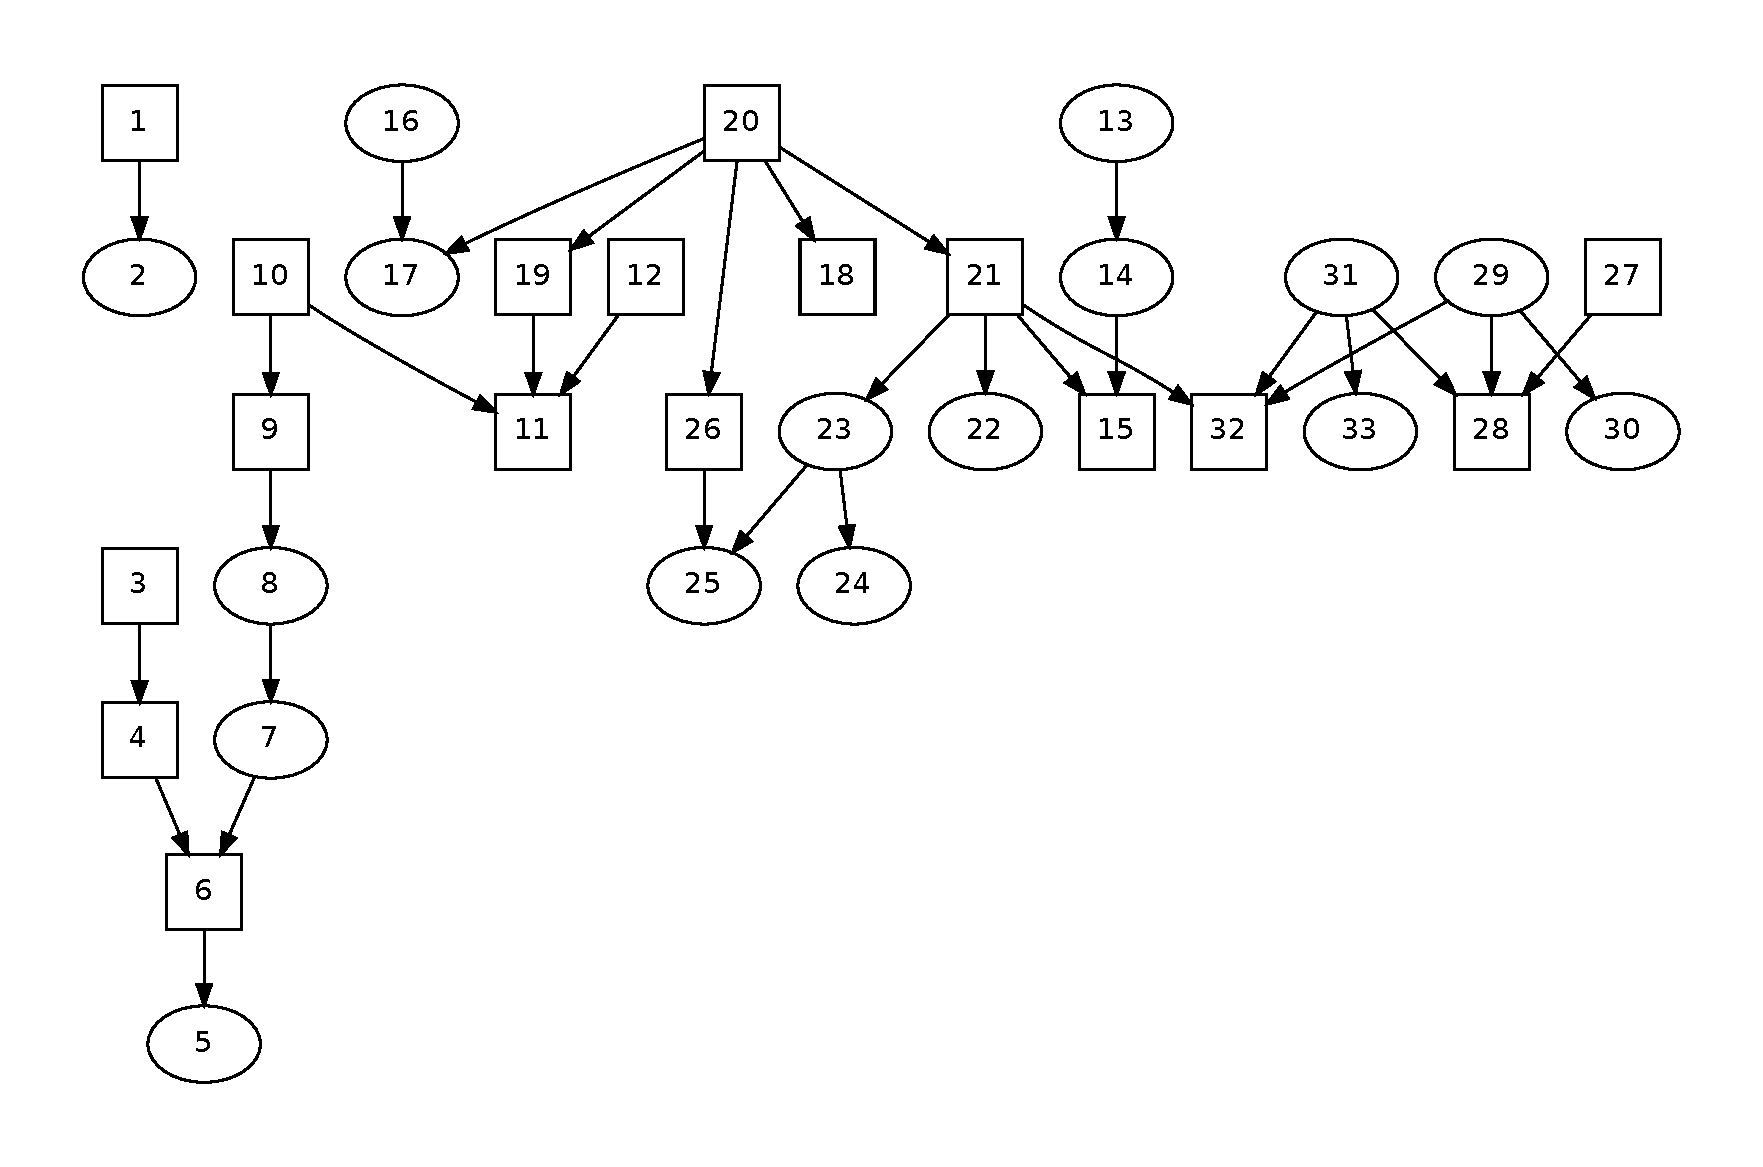
\includegraphics{var33_MASTER}
\vspace{-1.0cm}
\caption{Directed acyclic graph representation of the joint probability distribution which generated data set {\tt var33} which is included with {\tt abn}. The square nodes are categorical (binary) and the oval nodes continuous variables.} \label{fig1}
\end{figure}
shows the structure of the distribution which generated the data set {\tt var33} included with {\tt abn}. This diagram was created using the {\tt tographviz()} function of {\tt abn} (see later examples) which translates the matrix which defines a network - a directed acyclic graph - into a text file of suitable format for processing in Graphviz, where this processing was done outside of {\tt R}. Graphviz is freely available and operates on most platforms and can be downloaded from {\tt www.graphviz.org}, there is also an R package which interfaces to Graphviz available from the Bioconductor project (requires an installation of Graphviz). 

\section{Fitting a single BN model to data}
In the next sections we illustrate how to fit a BN model to different kinds of data. The main purpose of BN structure discovery is to estimate the joint dependency structure of the random variables in the available data, and this is achieved by heuristically searching for optimal models and comparing their goodness of fit using Bayes factors. It is assumed that all structures are equally supported in the absence of any data - an uniformative prior on structures - and so comparing Bayes factors collapses to comparing the marginal likelihoods which is done on a log scale. The log marginal likelihood for a BN is typically referred to as the network score. 

\subsection{Fitting a BN model to categorical data} \label{sec1}
A conjugate Bayesian network applied to categorical data is the classical application of Bayesian network analysis. Here the data are considered as a contingency table of frequency counts and the model describes conditional dependencies between different cells. Note these are not additive models. 

The function {\tt fitbn(data.df, dag.m, prior.obs.per.node=NULL, useK2=FALSE, ...)}\\ fits a multinomial conjugate BN model to the data in {\tt data.df} where the model structure is defined in matrix {\tt dag.m}. There are two choices of priors/goodness of fit metrics; the BDe metric and the K2 metric (see \citeauthor{HECKERMAN1995} \citeyear{HECKERMAN1995}). In brief, in the BDeu metric it is assumed that a number, {\tt prior.obs.per.node}, of prior observations have been observed at each node and these are uniformly distributed across all the hyperparameters at each node. For example in Figure \ref{fig1}, node 4 is conditionally dependent upon node 3, these are binary nodes and the parameters to be estimated are $P(v4=T|v3=T)$ and $P(v4=T|v3=F)$ where each of these has a Beta distributed prior of $Beta(\alpha_1,\alpha_2)$. Suppose {\tt prior.obs.per.node}=16, then with the BDeu metric we have a prior of $Beta(4,4)$ for each of these two parameters - note that $4+4+4+4=16$. Similarly, if there were two parents for node 4 then there would be four parameters to estimate (assuming both parents were binary) and in this case the prior for each parameter would be $Beta(2,2)$ where again the sum of the hyperparameters equals 16. In contrast, in the K2 metric each and every parameter has a flat prior of $Beta(1,1)$ for binary nodes and Dirichlet $Dir(1,\dots,1)$ for multinomial nodes. An advantage of the BDeu metric is that it is likelihood equivalent and so DAGs which are probabilistically equivalent will have identical BDeu network scores. The K2 metric, however, uses identical uninformative priors for each and every parameter which may also be desirable, but in which case the network scores for probabilistic identical networks may differ (although in practice such differences may be small) as the K2 metric is not likelihood equivalent. In {\tt fitbn}, if the {\tt useK2} argument is {\tt TRUE} then {\tt prior.obs.per.node} is ignored. 

The following code fits a network to the subset of the variables from {\tt var33} which are categorical. In this data these are all binary but {\tt fitbn} works analogously for multinomial variables. Note that all categorical variables should be set as factors.     
\begin{Schunk}
\begin{Sinput}
> library(abn);# load library
> bin.nodes<-c(1,3,4,6,9,10,11,12,15,18,19,20,21,26,27,28,32); 
> var33.cat<-var33[,bin.nodes];#categorical nodes only
> mydag<-matrix(c(
+                  0,0,0,0,0,0,0,0,0,0,0,0,0,0,0,0,0, #v1
+                  0,0,0,0,0,0,0,0,0,0,0,0,0,0,0,0,0, #v3
+                  0,0,0,0,0,0,0,0,0,0,0,0,0,0,0,0,0, #v4  
+                  0,0,0,0,0,0,0,0,0,0,0,0,0,0,0,0,0, #v6  
+                  0,0,0,0,0,0,0,0,0,0,0,0,0,0,0,0,0, #v9  
+                  0,0,0,0,0,0,0,0,0,0,0,0,0,0,0,0,0, #v10  
+                  0,0,0,0,0,0,0,0,0,0,0,0,0,0,0,0,0, #v11  
+                  0,0,0,0,0,0,0,0,0,0,0,0,0,0,0,0,0, #v12  
+                  0,0,0,0,0,0,0,0,0,0,0,0,0,0,0,0,0, #v15  
+                  0,0,0,0,0,0,0,0,0,0,0,0,0,0,0,0,0, #v18 
+                  0,0,0,0,0,0,0,0,0,0,0,0,0,0,0,0,0, #v19
+                  0,0,0,0,0,0,0,0,0,0,0,0,0,0,0,0,0, #v20 
+                  0,0,0,0,0,0,0,0,0,0,0,0,0,0,0,0,0, #v21 
+                  0,0,0,0,0,0,0,0,0,0,0,0,0,0,0,0,0, #v26 
+                  0,0,0,0,0,0,0,0,0,0,0,0,0,0,0,0,0, #v27 
+                  0,0,0,0,0,0,0,0,0,0,0,0,0,0,0,0,0, #v28 
+                  0,0,0,0,0,0,0,0,0,0,0,0,0,0,0,0,0  #v32 
+               ),byrow=TRUE,ncol=17); 
> colnames(mydag)<-rownames(mydag)<-names(var33.cat);#set names
> ## now fit the model defined in mydag - full independence model
> fitbn (data.df=var33.cat, dag.m=mydag,useK2=TRUE);
\end{Sinput}
\begin{Soutput}
[1] -2807.897
\end{Soutput}
\begin{Sinput}
> # this is the network score goodness of fit = log marginal likelihood
\end{Sinput}
\end{Schunk}
The structure of the network definition matrix is where each row is a ``child'' and each column is its ``parents'', where a {\tt 1} denotes a parent (or arc) is present. Now lets fit a model with some conditional dependencies, for example where {\tt v11} is conditionally dependent upon {\tt v12} and {\tt v10}, and {\tt v4} is conditionally dependent upon {\tt v3}.
\begin{Schunk}
\begin{Sinput}
> # now fit model with some conditional dependencies let v11 
> ## depend jointly on v12 and v10
> mydag["v11","v12"]<-1;
> mydag["v11","v10"]<-1;
> ## let v4 depend on v3
> mydag["v4","v3"]<-1;
> fitbn (data.df=var33.cat, dag.m=mydag,useK2=TRUE);
\end{Sinput}
\begin{Soutput}
[1] -2794.079
\end{Soutput}
\begin{Sinput}
> # network score for a model with conditional independence
\end{Sinput}
\end{Schunk}
The network score is considerably improved and therefore suggests support for these new structural features. To produce a visual description of the model then we can export to graphviz as follows
\begin{Schunk}
\begin{Sinput}
> tographviz(dag=mydag,data.df=var33.cat,outfile="mydag.dot");#create file
> # mydag.dot can then be processed with graphviz
> # unix shell "dot -Tpdf mydag.dot -o mydag.pdf" or use gedit if on Windows
\end{Sinput}
\end{Schunk}

\begin{figure}[htb]
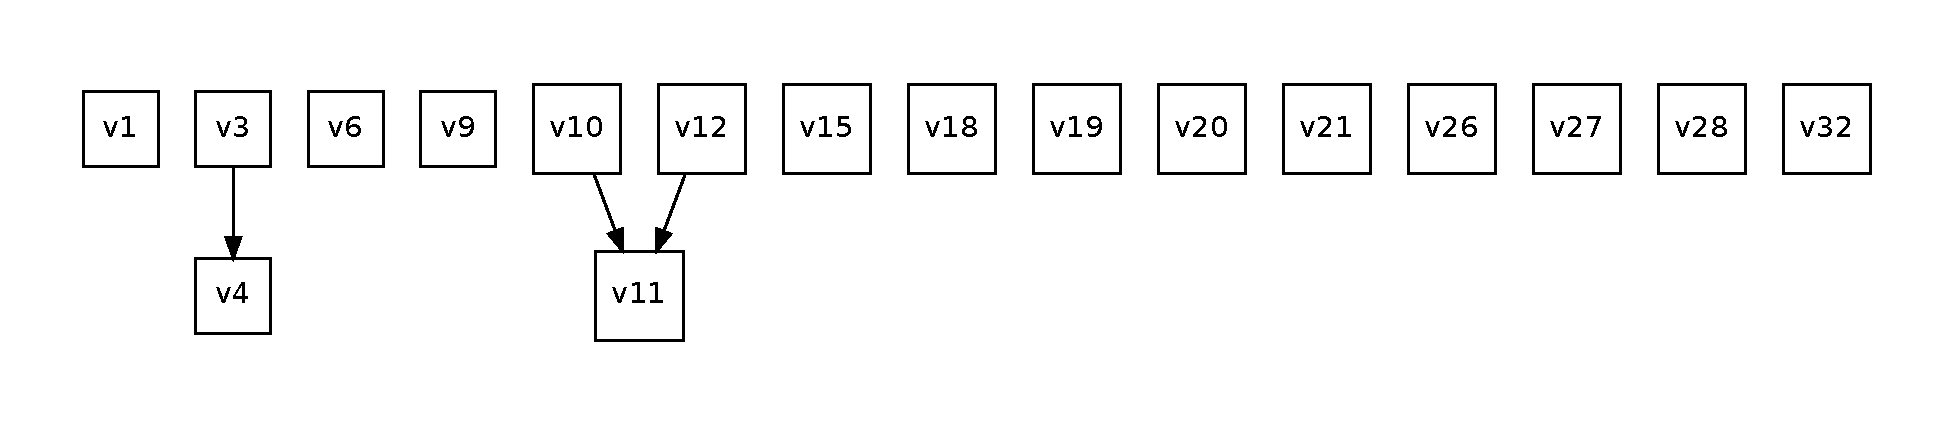
\includegraphics{mydag}
\vspace{-1.0cm}
\caption{Directed acyclic graph {\tt mydag} created using {\tt tographviz()} and Graphviz} \label{fig2}
\end{figure}
In {\tt tographviz()} the {\tt data.df} argument is used to determine whether the variable is a factor or not, where factors are displayed as squares and non-factors as ovals. To use the full range of visual Graphviz options simply use the file created by {\tt tographviz()} as a starting point and manually edit this in a text editor before running through {\tt dot} or one of the other Graphviz layout processors.

\subsection{Fitting an additive BN model to categorical data} \label{sec2}
An additive BN model for categorical data can be constructed by considering each individual variable as a logistic regression of the other variables in the data, and hence the network model comprises of many combinations of local logistic regressions. The parameters in this model are the additive terms in a usual logistic regression and independent Gaussian priors are assumed for each covariate. Note that the variables here must all be binary, and so all multinomial variables need to be split into separate binary factors (and added to the original data.frame) in order to form the network model. This is analogous to forming the design matrix in a conventional additive model analysis. Similarly, interaction terms can be added by including appropriate additional columns in the data.frame. In these models the log marginal likelihood (network score) is estimated using Laplace approximations at each node. Hyperparameters for the means and variances in the Gaussian priors are fixed at zero and 1000 respectively, and other values can be given explicitly in the call to {\tt fitabn} but this is not recommended without good reason.

To fit an additive model use {\tt fitabn(data.df,dag.m, ...)}. In the following code we fit first the independence model with no arcs and then the same dependence model as above. Turning on {\tt verbose=TRUE} simply gives the individual log marginal likelihoods for each node (n.b. the numbering is that used internally and simply denotes the variables in the data.frame from left to right).
\begin{Schunk}
\begin{Sinput}
> ## move back to independence model
> mydag["v11","v12"]<-0;mydag["v11","v10"]<-0;mydag["v4","v3"]<-0;
> fitabn (data.df=var33.cat,dag.m=mydag,verbose=TRUE);
\end{Sinput}
\begin{Soutput}
Binary node=0 score=-178.004211
Binary node=1 score=-178.414495
Binary node=2 score=-168.248843
Binary node=3 score=-102.675919
Binary node=4 score=-167.644794
Binary node=5 score=-178.679732
Binary node=6 score=-174.534904
Binary node=7 score=-178.293870
Binary node=8 score=-143.134495
Binary node=9 score=-173.338554
Binary node=10 score=-174.152823
Binary node=11 score=-177.448401
Binary node=12 score=-177.448401
Binary node=13 score=-167.644794
Binary node=14 score=-178.735970
Binary node=15 score=-174.900353
Binary node=16 score=-163.647060

   #################################################################
   ###      log marginal likelihood for Model: -2856.9476195086
   #################################################################
[1] -2856.948
\end{Soutput}
\begin{Sinput}
> # now fit the model with some conditional dependencies 
> mydag["v11","v12"]<-1;mydag["v11","v10"]<-1;mydag["v4","v3"]<-1;
> fitabn (data.df=var33.cat, dag.m=mydag,verbose=TRUE);
\end{Sinput}
\begin{Soutput}
Binary node=0 score=-178.004211
Binary node=1 score=-178.414495
Binary node=2 score=-166.945426
Binary node=3 score=-102.675919
Binary node=4 score=-167.644794
Binary node=5 score=-178.679732
Binary node=6 score=-168.972182
Binary node=7 score=-178.293870
Binary node=8 score=-143.134495
Binary node=9 score=-173.338554
Binary node=10 score=-174.152823
Binary node=11 score=-177.448401
Binary node=12 score=-177.448401
Binary node=13 score=-167.644794
Binary node=14 score=-178.735970
Binary node=15 score=-174.900353
Binary node=16 score=-163.647060

   #################################################################
   ###      log marginal likelihood for Model: -2850.0814800302
   #################################################################
[1] -2850.081
\end{Soutput}
\begin{Sinput}
> # network score for a model with conditional independence
\end{Sinput}
\end{Schunk}

\subsection{Fitting an additive BN model to continuous data} \label{sec3} 
We now consider analogous models to those in Section \ref{sec2} but where the network comprises of Gaussian linear regressions rather than logistic regressions. The structure of these models again assumes independent Gaussian priors for each of the coefficients in the additive components for the mean response at each node (with hyper means = 0 and hyper variances = 1000). The Gaussian response distribution is parameterized in terms of precision $(1/\sigma^2)$, and independent Gamma priors are used with shape=0.001 and scale=1/0.001 (where these are as defined in the {\tt rgamma} help page). By default, each variable in the data.frame is standardised to a mean of zero and standard deviation of one, this has no effect on the identification of dependencies between variables. 
\begin{Schunk}
\begin{Sinput}
> var33.cts<-var33[,-bin.nodes];#drop categorical nodes
> mydag<-matrix(c(
+                  0,0,0,0,0,0,0,0,0,0,0,0,0,0,0,0, #v2
+                  0,0,0,0,0,0,0,0,0,0,0,0,0,0,0,0, #v5  
+                  0,0,0,0,0,0,0,0,0,0,0,0,0,0,0,0, #v7  
+                  0,0,0,0,0,0,0,0,0,0,0,0,0,0,0,0, #v8 
+                  0,0,0,0,0,0,0,0,0,0,0,0,0,0,0,0, #v13  
+                  0,0,0,0,0,0,0,0,0,0,0,0,0,0,0,0, #v14  
+                  0,0,0,0,0,0,0,0,0,0,0,0,0,0,0,0, #v16  
+                  0,0,0,0,0,0,0,0,0,0,0,0,0,0,0,0, #v17  
+                  0,0,0,0,0,0,0,0,0,0,0,0,0,0,0,0, #v22 
+                  0,0,0,0,0,0,0,0,0,0,0,0,0,0,0,0, #v23
+                  0,0,0,0,0,0,0,0,0,0,0,0,0,0,0,0, #v24 
+                  0,0,0,0,0,0,0,0,0,0,0,0,0,0,0,0, #v25 
+                  0,0,0,0,0,0,0,0,0,0,0,0,0,0,0,0, #v29 
+                  0,0,0,0,0,0,0,0,0,0,0,0,0,0,0,0, #v30 
+                  0,0,0,0,0,0,0,0,0,0,0,0,0,0,0,0, #v31 
+                  0,0,0,0,0,0,0,0,0,0,0,0,0,0,0,0  #v33 
+               ),byrow=TRUE,ncol=16); 
> colnames(mydag)<-rownames(mydag)<-names(var33.cts);#set names
> ## now fit the model defined in mydag - full independence
> fitabn (data.df=var33.cts,dag.m=mydag,verbose=TRUE);
\end{Sinput}
\begin{Soutput}
Gaussian node=0 score=-368.856543
Gaussian node=1 score=-368.856543
Gaussian node=2 score=-368.856543
Gaussian node=3 score=-368.856543
Gaussian node=4 score=-368.856543
Gaussian node=5 score=-368.856543
Gaussian node=6 score=-368.856543
Gaussian node=7 score=-368.856543
Gaussian node=8 score=-368.856543
Gaussian node=9 score=-368.856543
Gaussian node=10 score=-368.856543
Gaussian node=11 score=-368.856543
Gaussian node=12 score=-368.856543
Gaussian node=13 score=-368.856543
Gaussian node=14 score=-368.856543
Gaussian node=15 score=-368.856543

   #################################################################
   ###      log marginal likelihood for Model: -5901.7046880253
   #################################################################
[1] -5901.705
\end{Soutput}
\begin{Sinput}
> ## uses default priors of N(mu=0,var=1000), 1/var=Gamma(0.001,1/0.001)
> # this is the network score goodness of fit = log marginal likelihood
\end{Sinput}
\end{Schunk}
Now fit a model with conditional independencies, for example 
\begin{Schunk}
\begin{Sinput}
> # now fit model with some conditional dependencies let v33 
> ## depend on v31, and v24 depend on 23, and v14 depend on v13
> mydag["v33","v31"]<-1;
> mydag["v24","v23"]<-1;
> mydag["v14","v13"]<-1;
> fitabn (data.df=var33.cts, dag.m=mydag,verbose=TRUE);
\end{Sinput}
\begin{Soutput}
Gaussian node=0 score=-368.856543
Gaussian node=1 score=-368.856543
Gaussian node=2 score=-368.856543
Gaussian node=3 score=-368.856543
Gaussian node=4 score=-368.856543
Gaussian node=5 score=-292.856329
Gaussian node=6 score=-368.856543
Gaussian node=7 score=-368.856543
Gaussian node=8 score=-368.856543
Gaussian node=9 score=-368.856543
Gaussian node=10 score=-288.517729
Gaussian node=11 score=-368.856543
Gaussian node=12 score=-368.856543
Gaussian node=13 score=-368.856543
Gaussian node=14 score=-368.856543
Gaussian node=15 score=-282.320155

   #################################################################
   ###      log marginal likelihood for Model: -5658.8292728846
   #################################################################
[1] -5658.829
\end{Soutput}
\begin{Sinput}
> # network score for a model with conditional independence
> tographviz(dag=mydag,data.df=var33.cts,outfile="mydagcts.dot");#create file
> # mydag.dot can then be processed with graphviz
> # unix shell "dot -Tpdf mydagcts.dot -o mydagcts.pdf" or use gedit if on Windows
\end{Sinput}
\end{Schunk}
\begin{figure}[htb]
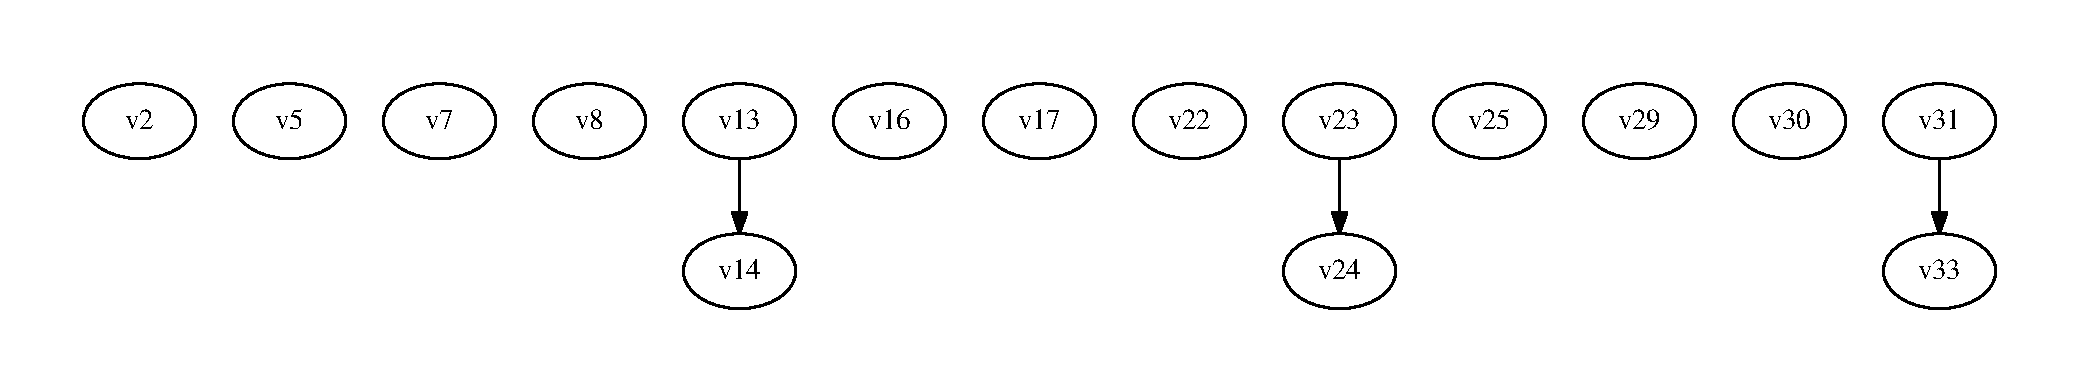
\includegraphics{mydagcts}
\vspace{-1.0cm}
\caption{Directed acyclic graph {\tt mydag} for continuous variables only created using {\tt tographviz()} and Graphviz} \label{fig3}
\end{figure}


\subsection{Fitting an additive BN model to mixed data} \label{sec4}
To conclude the fitting of a single pre-specified model to data, e.g. based on expert opinion, we consider an additive BN model which comprises both binary and Gaussian nodes and this comprises of a combination of Binomial (logistic) and Gaussian linear models. Again {\tt fitabn()} is used and the code is almost identical to the previous examples. 
\begin{Schunk}
\begin{Sinput}
> mydag<-matrix(c(
+ 0,0,0,0,0,0,0,0,0,0,0,0,0,0,0,0,0,0,0,0,0,0,0,0,0,0,0,0,0,0,0,0,0,#1
+ 0,0,0,0,0,0,0,0,0,0,0,0,0,0,0,0,0,0,0,0,0,0,0,0,0,0,0,0,0,0,0,0,0,#2  
+ 0,0,0,0,0,0,0,0,0,0,0,0,0,0,0,0,0,0,0,0,0,0,0,0,0,0,0,0,0,0,0,0,0,#3  
+ 0,0,0,0,0,0,0,0,0,0,0,0,0,0,0,0,0,0,0,0,0,0,0,0,0,0,0,0,0,0,0,0,0,#4  
+ 0,0,0,0,0,0,0,0,0,0,0,0,0,0,0,0,0,0,0,0,0,0,0,0,0,0,0,0,0,0,0,0,0,#5  
+ 0,0,0,0,0,0,0,0,0,0,0,0,0,0,0,0,0,0,0,0,0,0,0,0,0,0,0,0,0,0,0,0,0,#6  
+ 0,0,0,0,0,0,0,0,0,0,0,0,0,0,0,0,0,0,0,0,0,0,0,0,0,0,0,0,0,0,0,0,0,#7  
+ 0,0,0,0,0,0,0,0,0,0,0,0,0,0,0,0,0,0,0,0,0,0,0,0,0,0,0,0,0,0,0,0,0,#8  
+ 0,0,0,0,0,0,0,0,0,0,0,0,0,0,0,0,0,0,0,0,0,0,0,0,0,0,0,0,0,0,0,0,0,#9  
+ 0,0,0,0,0,0,0,0,0,0,0,0,0,0,0,0,0,0,0,0,0,0,0,0,0,0,0,0,0,0,0,0,0,#10 
+ 0,0,0,0,0,0,0,0,0,0,0,0,0,0,0,0,0,0,0,0,0,0,0,0,0,0,0,0,0,0,0,0,0,#11 
+ 0,0,0,0,0,0,0,0,0,0,0,0,0,0,0,0,0,0,0,0,0,0,0,0,0,0,0,0,0,0,0,0,0,#12 
+ 0,0,0,0,0,0,0,0,0,0,0,0,0,0,0,0,0,0,0,0,0,0,0,0,0,0,0,0,0,0,0,0,0,#13 
+ 0,0,0,0,0,0,0,0,0,0,0,0,0,0,0,0,0,0,0,0,0,0,0,0,0,0,0,0,0,0,0,0,0,#14 
+ 0,0,0,0,0,0,0,0,0,0,0,0,0,0,0,0,0,0,0,0,0,0,0,0,0,0,0,0,0,0,0,0,0,#15 
+ 0,0,0,0,0,0,0,0,0,0,0,0,0,0,0,0,0,0,0,0,0,0,0,0,0,0,0,0,0,0,0,0,0,#16 
+ 0,0,0,0,0,0,0,0,0,0,0,0,0,0,0,0,0,0,0,0,0,0,0,0,0,0,0,0,0,0,0,0,0,#17 
+ 0,0,0,0,0,0,0,0,0,0,0,0,0,0,0,0,0,0,0,0,0,0,0,0,0,0,0,0,0,0,0,0,0,#18 
+ 0,0,0,0,0,0,0,0,0,0,0,0,0,0,0,0,0,0,0,0,0,0,0,0,0,0,0,0,0,0,0,0,0,#19 
+ 0,0,0,0,0,0,0,0,0,0,0,0,0,0,0,0,0,0,0,0,0,0,0,0,0,0,0,0,0,0,0,0,0,#20 
+ 0,0,0,0,0,0,0,0,0,0,0,0,0,0,0,0,0,0,0,0,0,0,0,0,0,0,0,0,0,0,0,0,0,#21 
+ 0,0,0,0,0,0,0,0,0,0,0,0,0,0,0,0,0,0,0,0,0,0,0,0,0,0,0,0,0,0,0,0,0,#22 
+ 0,0,0,0,0,0,0,0,0,0,0,0,0,0,0,0,0,0,0,0,0,0,0,0,0,0,0,0,0,0,0,0,0,#23 
+ 0,0,0,0,0,0,0,0,0,0,0,0,0,0,0,0,0,0,0,0,0,0,0,0,0,0,0,0,0,0,0,0,0,#24 
+ 0,0,0,0,0,0,0,0,0,0,0,0,0,0,0,0,0,0,0,0,0,0,0,0,0,0,0,0,0,0,0,0,0,#25 
+ 0,0,0,0,0,0,0,0,0,0,0,0,0,0,0,0,0,0,0,0,0,0,0,0,0,0,0,0,0,0,0,0,0,#26 
+ 0,0,0,0,0,0,0,0,0,0,0,0,0,0,0,0,0,0,0,0,0,0,0,0,0,0,0,0,0,0,0,0,0,#27 
+ 0,0,0,0,0,0,0,0,0,0,0,0,0,0,0,0,0,0,0,0,0,0,0,0,0,0,0,0,0,0,0,0,0,#28 
+ 0,0,0,0,0,0,0,0,0,0,0,0,0,0,0,0,0,0,0,0,0,0,0,0,0,0,0,0,0,0,0,0,0,#29 
+ 0,0,0,0,0,0,0,0,0,0,0,0,0,0,0,0,0,0,0,0,0,0,0,0,0,0,0,0,0,0,0,0,0,#30
+ 0,0,0,0,0,0,0,0,0,0,0,0,0,0,0,0,0,0,0,0,0,0,0,0,0,0,0,0,0,0,0,0,0,#31
+ 0,0,0,0,0,0,0,0,0,0,0,0,0,0,0,0,0,0,0,0,0,0,0,0,0,0,0,0,0,0,0,0,0,#32 
+ 0,0,0,0,0,0,0,0,0,0,0,0,0,0,0,0,0,0,0,0,0,0,0,0,0,0,0,0,0,0,0,0,0 #33
+                                                ),byrow=TRUE,ncol=33); 
> colnames(mydag)<-rownames(mydag)<-names(var33);#set names
> ## now fit the model defined in mydag - full independence
> fitabn (data.df=var33,dag.m=mydag,verbose=TRUE);
\end{Sinput}
\begin{Soutput}
Binary node=0 score=-178.004211
Gaussian node=1 score=-368.856543
Binary node=2 score=-178.414495
Binary node=3 score=-168.248843
Gaussian node=4 score=-368.856543
Binary node=5 score=-102.675919
Gaussian node=6 score=-368.856543
Gaussian node=7 score=-368.856543
Binary node=8 score=-167.644794
Binary node=9 score=-178.679732
Binary node=10 score=-174.534904
Binary node=11 score=-178.293870
Gaussian node=12 score=-368.856543
Gaussian node=13 score=-368.856543
Binary node=14 score=-143.134495
Gaussian node=15 score=-368.856543
Gaussian node=16 score=-368.856543
Binary node=17 score=-173.338554
Binary node=18 score=-174.152823
Binary node=19 score=-177.448401
Binary node=20 score=-177.448401
Gaussian node=21 score=-368.856543
Gaussian node=22 score=-368.856543
Gaussian node=23 score=-368.856543
Gaussian node=24 score=-368.856543
Binary node=25 score=-167.644794
Binary node=26 score=-178.735970
Binary node=27 score=-174.900353
Gaussian node=28 score=-368.856543
Gaussian node=29 score=-368.856543
Gaussian node=30 score=-368.856543
Binary node=31 score=-163.647060
Gaussian node=32 score=-368.856543

   #################################################################
   ###      log marginal likelihood for Model: -8758.6523075339
   #################################################################
[1] -8758.652
\end{Soutput}
\end{Schunk}
We now fit a BN model which has the same structure as the joint distribution used to generate the data and then create a visual graph of this model
\begin{Schunk}
\begin{Sinput}
> # define a model with many independencies
> mydag[2,1]<-1;
> mydag[4,3]<-1;
> mydag[6,4]<-1; mydag[6,7]<-1;
> mydag[5,6]<-1;
> mydag[7,8]<-1;  
> mydag[8,9]<-1;
> mydag[9,10]<-1;
> mydag[11,10]<-1; mydag[11,12]<-1; mydag[11,19]<-1;
> mydag[14,13]<-1;
> mydag[17,16]<-1;mydag[17,20]<-1;
> mydag[15,14]<-1; mydag[15,21]<-1;
> mydag[18,20]<-1;
> mydag[19,20]<-1;
> mydag[21,20]<-1;
> mydag[22,21]<-1;
> mydag[23,21]<-1;
> mydag[24,23]<-1;
> mydag[25,23]<-1; mydag[25,26]<-1;
> mydag[26,20]<-1;
> mydag[33,31]<-1;
> mydag[33,31]<-1;
> mydag[32,21]<-1; mydag[32,31]<-1;mydag[32,29]<-1;    
> mydag[30,29]<-1;
> mydag[28,27]<-1; mydag[28,29]<-1;mydag[28,31]<-1;       
> fitabn (data.df=var33, dag.m=mydag);
\end{Sinput}
\begin{Soutput}
[1] -7977.915
\end{Soutput}
\begin{Sinput}
> # network score for a model with conditional independence
> tographviz(dag=mydag,data.df=var33,outfile="mydag_all.dot");#create file
> # mydag.dot can then be processed with graphviz
> # unix shell "dot -Tpdf mydag_all.dot -o mydag_all.pdf" or use gedit if on Windows
\end{Sinput}
\end{Schunk}
\begin{figure}[htb]
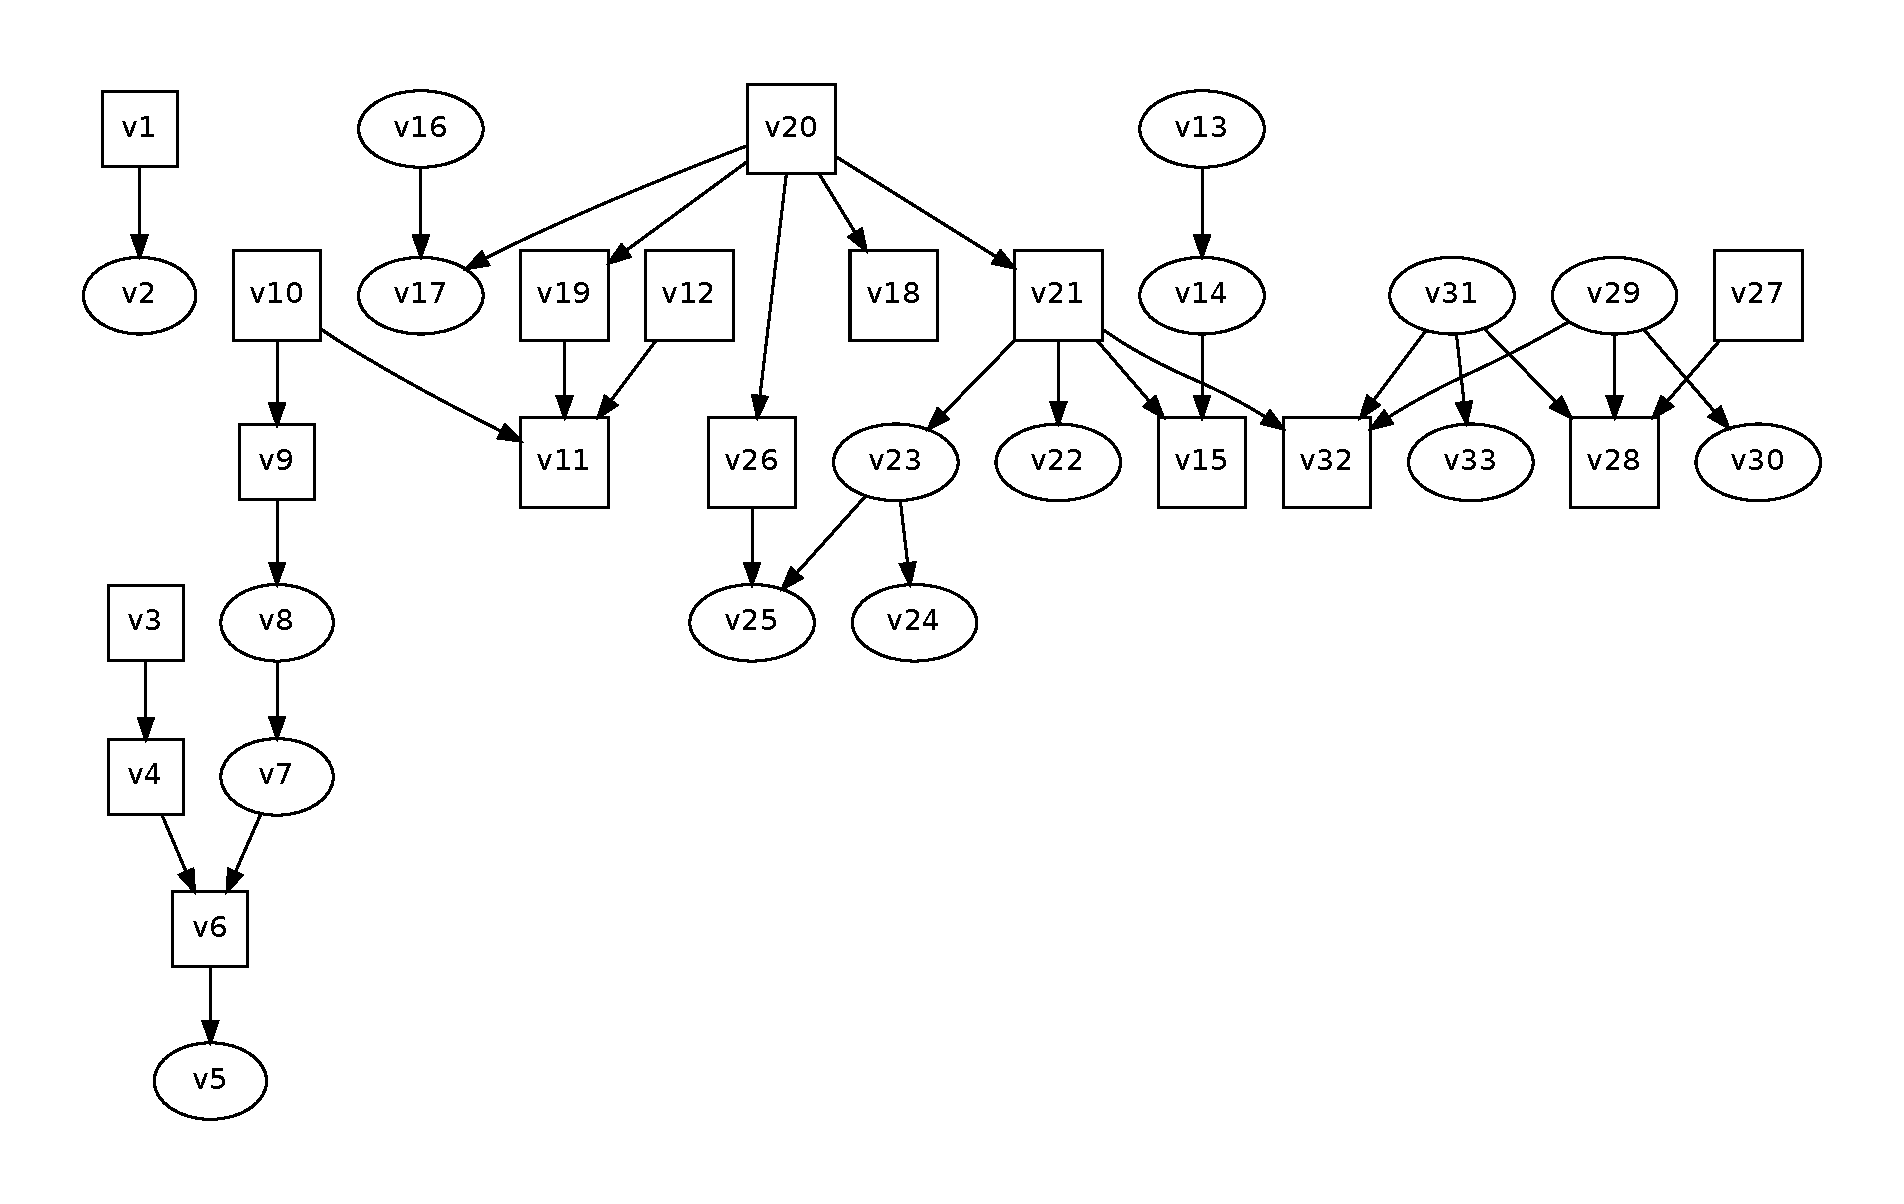
\includegraphics{mydag_all}
\vspace{-1.0cm}
\caption{Directed acyclic graph {\tt mydag} for mixed continuous and discrete variables} \label{fig4}
\end{figure}

\subsection{Model fitting validation}
In order to validate the conjugate models, network scores for both overall networks and individual nodes using the Bayesian Dirichlet equivalence uniform (BDeu) metric were compared with the {\tt deal} library available from {\tt CRAN}. This metric can be used by {\tt useK2=FALSE} and providing an explicit value for {\tt prior.obs.per.node}. A wide range of models for multinomial data were compared and these were always identical to those values produced by {\tt deal}. To validate the additive models for mixed binary and Gaussian models, estimates of the posterior distributions for the model parameters using Laplace approximations were compared with those estimated using Markov chain Monte Carlo. These were always in very close agreement for the range of models and data examined. This is an indirect validation of the Laplace estimate of the network score, e.g. if the posterior densities match closely then this implies that the denominator (the marginal likelihood - network score) must also be accurately estimated, as a ``gold standard'' estimate of the network score is generally unavailable for such non-conjugate models. 

\section{Searching for Optimal Models} \label{sec5}
The key objective of the {\tt abn} library is to enable estimation of statistical dependencies in data comprising of multiple variables - that is, find a DAG which is robust and representative of the dependency structure of the (unknown) stochastic system which generated the observed data. The challenge here is that with such a vast model space it is impossible to enumerate over all possible DAGs, and there may be very many different DAGs with similar goodness of fit. In the next sections we first consider searching for categorical (conjugate) BN models, then additive (non-conjugate) models. 

\subsection{Single search for optimal BN model from categorical data}
To run a single search heuristic use {\tt searchbn()}. This commences from a randomly created DAG which is constructed by randomly adding arcs to an empty network until either {\tt init.permuts} arcs are present or else all possible arcs have been tried. If a start DAG is given which contains arcs then {\tt init.permuts} is in addition to those arcs already present. The function {\tt searchbn()} then searches stepwise from the initial random network for an improved structure, where three stepwise operations are possible: i) add an arc; ii) remove and arc; or iii) reverse and arc. The stepwise search is subject to a number of conditions, firstly only moves that do not generate a cycle are permitted, secondly, a parent limit is imposed which fixes the maximum number of parents which each child node can have (arcs go from parent to child), and thirdly it is possible to ban or retain arcs. If provided, {\tt banned.m} is a matrix which defines arcs that are not allowed to be considered in the search process (or in the creation of the initial random network). Similarly, {\tt retain.m} includes arcs which must always be included in any model. It is also possible to specific an explicit starting matrix, {\tt start.m} and if using a retain matrix then {\tt start.m} should contain at least all those arcs present in {\tt retain.m}. Note that only very rudimentary checking is done to make sure that the ban, retain and start networks - if user supplied - are not contradictory.

To improve the computational performance of {\tt searchbn()} by default a node cache is used. Rather than re-calculate the score for each individual node in the network (the overall network score is the product of all the scores for the individual nodes) the score for each unique node found during the search is stored in a lookup table. This can make very significant improvements in speed and the default is for a search to terminate prematurely if the node cache is exceeded. This behaviour can be turned off by {\tt enforce.db.size=FALSE}, and so once the cache is exceeded then the search will proceed but may now incur duplicate calculation of nodes. It is generally advisable to use a sufficiently large value for {\tt db.size} to avoid this (a warning will appear to say this limit has been reached if {\tt enforce.db.size=FALSE}). 

\begin{Schunk}
\begin{Sinput}
> bin.nodes<-c(1,3,4,6,9,10,11,12,15,18,19,20,21,26,27,28,32); 
> var33.cat<-var33[,bin.nodes];#categorical nodes only
> mydag<-matrix(c(
+                  0,0,0,0,0,0,0,0,0,0,0,0,0,0,0,0,0, #v1
+                  0,0,0,0,0,0,0,0,0,0,0,0,0,0,0,0,0, #v3
+                  0,0,0,0,0,0,0,0,0,0,0,0,0,0,0,0,0, #v4  
+                  0,0,0,0,0,0,0,0,0,0,0,0,0,0,0,0,0, #v6  
+                  0,0,0,0,0,0,0,0,0,0,0,0,0,0,0,0,0, #v9  
+                  0,0,0,0,0,0,0,0,0,0,0,0,0,0,0,0,0, #v10  
+                  0,0,0,0,0,0,0,0,0,0,0,0,0,0,0,0,0, #v11  
+                  0,0,0,0,0,0,0,0,0,0,0,0,0,0,0,0,0, #v12  
+                  0,0,0,0,0,0,0,0,0,0,0,0,0,0,0,0,0, #v15  
+                  0,0,0,0,0,0,0,0,0,0,0,0,0,0,0,0,0, #v18 
+                  0,0,0,0,0,0,0,0,0,0,0,0,0,0,0,0,0, #v19
+                  0,0,0,0,0,0,0,0,0,0,0,0,0,0,0,0,0, #v20 
+                  0,0,0,0,0,0,0,0,0,0,0,0,0,0,0,0,0, #v21 
+                  0,0,0,0,0,0,0,0,0,0,0,0,0,0,0,0,0, #v26 
+                  0,0,0,0,0,0,0,0,0,0,0,0,0,0,0,0,0, #v27 
+                  0,0,0,0,0,0,0,0,0,0,0,0,0,0,0,0,0, #v28 
+                  0,0,0,0,0,0,0,0,0,0,0,0,0,0,0,0,0  #v32 
+               ),byrow=TRUE,ncol=17); 
> colnames(mydag)<-rownames(mydag)<-names(var33.cat);#set names
> ## create empty DAGs
> banned.cat<-matrix(rep(0,dim(var33.cat)[2]^2),ncol=dim(var33.cat)[2]);
> colnames(banned.cat)<-rownames(banned.cat)<-names(var33.cat);#set names
> retain.cat<-matrix(rep(0,dim(var33.cat)[2]^2),ncol=dim(var33.cat)[2]);
> colnames(retain.cat)<-rownames(retain.cat)<-names(var33.cat);#set names
> start.cat<-matrix(rep(0,dim(var33.cat)[2]^2),ncol=dim(var33.cat)[2]);
> colnames(start.cat)<-rownames(start.cat)<-names(var33.cat);#set names
> myres<-searchbn(data.df=var33.cat,
+                 banned.m=banned.cat,
+                 retain.m=retain.cat,
+                 start.m=start.cat,
+                 useK2=TRUE,max.parents=2,init.permuts=0,db.size=1000);
\end{Sinput}
\begin{Soutput}
initial network: (log) network score = -2807.897043
search iteration...1 new score=-2792.611588
search iteration...2 new score=-2780.682103
search iteration...3 new score=-2770.481097
search iteration...4 new score=-2762.389571
search iteration...5 new score=-2755.035383
search iteration...6 new score=-2748.571708
search iteration...7 new score=-2742.693551
search iteration...8 new score=-2738.549529
search iteration...9 new score=-2735.237539
search iteration...10 new score=-2732.236456
search iteration...11 new score=-2729.548455
search iteration...12 new score=-2726.874298
search iteration...13 new score=-2725.316377
search iteration...14 new score=-2723.833990
search iteration...15 new score=-2722.476497
search iteration...16 new score=-2721.757042
search iteration...17 new score=-2721.447508
search iteration...18 new score=-2721.167697
search iteration...19 new score=-2720.919301
search iteration...20 new score=-2720.739712
\end{Soutput}
\end{Schunk}

\subsection{Single search for optimal additive BN model from categorical data}
Running a single search heuristic for an additive BN uses {\tt searchabn()}, and is very similar to {\tt searchbn()}, the main difference is in the parameter prior specifications (as detailed above). Several additional arguments are available which relate to the numerical routines used in the Laplace approximation to calculate the network score. The defaults appear to work reasonably well in practice and if it is not possible to calculate a robust value for this approximation in any model, for example due to a singular design matrix at one or more nodes, then the model is simply assigned a log network score of $-\infty$ which effectively removes it from the model search.  

\begin{Schunk}
\begin{Sinput}
> ## just use default priors 
> myres.add<-searchabn(data.df=var33.cat,
+                  banned.m=banned.cat,
+                  retain.m=retain.cat,
+                  start.m=start.cat,
+                  max.parents=2, 
+                  init.permuts=0,db.size=1000,error.verbose=TRUE);
\end{Sinput}
\begin{Soutput}
initial network: (log) network score = -2856.947620
search iteration...1 new score=-2844.262707
search iteration...2 new score=-2835.074372
search iteration...3 new score=-2827.621507
search iteration...4 new score=-2822.271092
search iteration...5 new score=-2817.634782
search iteration...6 new score=-2813.767954
search iteration...7 new score=-2810.668296
search iteration...8 new score=-2809.364421
search iteration...9 new score=-2808.871702
search iteration...10 new score=-2808.745553
\end{Soutput}
\end{Schunk}

\subsection{Single search for optimal BN model for continuous data} \label{sec4a}
As above but for a network of Gaussian nodes.
\begin{Schunk}
\begin{Sinput}
> var33.cts<-var33[,-bin.nodes];#drop categorical nodes
> mydag<-matrix(c(
+                  0,0,0,0,0,0,0,0,0,0,0,0,0,0,0,0, #v2
+                  0,0,0,0,0,0,0,0,0,0,0,0,0,0,0,0, #v5  
+                  0,0,0,0,0,0,0,0,0,0,0,0,0,0,0,0, #v7  
+                  0,0,0,0,0,0,0,0,0,0,0,0,0,0,0,0, #v8 
+                  0,0,0,0,0,0,0,0,0,0,0,0,0,0,0,0, #v13  
+                  0,0,0,0,0,0,0,0,0,0,0,0,0,0,0,0, #v14  
+                  0,0,0,0,0,0,0,0,0,0,0,0,0,0,0,0, #v16  
+                  0,0,0,0,0,0,0,0,0,0,0,0,0,0,0,0, #v17  
+                  0,0,0,0,0,0,0,0,0,0,0,0,0,0,0,0, #v22 
+                  0,0,0,0,0,0,0,0,0,0,0,0,0,0,0,0, #v23
+                  0,0,0,0,0,0,0,0,0,0,0,0,0,0,0,0, #v24 
+                  0,0,0,0,0,0,0,0,0,0,0,0,0,0,0,0, #v25 
+                  0,0,0,0,0,0,0,0,0,0,0,0,0,0,0,0, #v29 
+                  0,0,0,0,0,0,0,0,0,0,0,0,0,0,0,0, #v30 
+                  0,0,0,0,0,0,0,0,0,0,0,0,0,0,0,0, #v31 
+                  0,0,0,0,0,0,0,0,0,0,0,0,0,0,0,0  #v33 
+               ),byrow=TRUE,ncol=16); 
> colnames(mydag)<-rownames(mydag)<-names(var33.cts);#set names
> banned.cts<-matrix(rep(0,dim(var33.cts)[2]^2),ncol=dim(var33.cts)[2]);
> colnames(banned.cts)<-rownames(banned.cts)<-names(var33.cts);#set names
> retain.cts<-matrix(rep(0,dim(var33.cts)[2]^2),ncol=dim(var33.cts)[2]);
> colnames(retain.cts)<-rownames(retain.cts)<-names(var33.cts);#set names
> start.cts<-matrix(rep(0,dim(var33.cts)[2]^2),ncol=dim(var33.cts)[2]);
> colnames(start.cts)<-rownames(start.cts)<-names(var33.cts);#set names
> #
> myres.add<-searchabn(data.df=var33.cts,
+                  banned.m=banned.cts,
+                  retain.m=retain.cts,
+                  start.m=start.cts,
+                  max.parents=2, 
+                  init.permuts=0,db.size=1000,error.verbose=TRUE);
\end{Sinput}
\begin{Soutput}
initial network: (log) network score = -5901.704688
search iteration...1 new score=-5815.168300
search iteration...2 new score=-5730.298710
search iteration...3 new score=-5649.959896
search iteration...4 new score=-5572.001806
search iteration...5 new score=-5496.001592
search iteration...6 new score=-5428.150967
search iteration...7 new score=-5376.806098
search iteration...8 new score=-5375.737019
\end{Soutput}
\end{Schunk}

\subsection{Single search for optimal additive BN model for mixed data}
Model searching for mixed data is again very similar to the previous examples. Note that in this example the parameter priors are specified explicitly (although those given are the same as the defaults). The {\tt +1} in the hyperparameter specification is because a constant term is included in the additive formulation for each node.

\begin{Schunk}
\begin{Sinput}
> mydag<-matrix(c(
+ 0,0,0,0,0,0,0,0,0,0,0,0,0,0,0,0,0,0,0,0,0,0,0,0,0,0,0,0,0,0,0,0,0,#1
+ 0,0,0,0,0,0,0,0,0,0,0,0,0,0,0,0,0,0,0,0,0,0,0,0,0,0,0,0,0,0,0,0,0,#2  
+ 0,0,0,0,0,0,0,0,0,0,0,0,0,0,0,0,0,0,0,0,0,0,0,0,0,0,0,0,0,0,0,0,0,#3  
+ 0,0,0,0,0,0,0,0,0,0,0,0,0,0,0,0,0,0,0,0,0,0,0,0,0,0,0,0,0,0,0,0,0,#4  
+ 0,0,0,0,0,0,0,0,0,0,0,0,0,0,0,0,0,0,0,0,0,0,0,0,0,0,0,0,0,0,0,0,0,#5  
+ 0,0,0,0,0,0,0,0,0,0,0,0,0,0,0,0,0,0,0,0,0,0,0,0,0,0,0,0,0,0,0,0,0,#6  
+ 0,0,0,0,0,0,0,0,0,0,0,0,0,0,0,0,0,0,0,0,0,0,0,0,0,0,0,0,0,0,0,0,0,#7  
+ 0,0,0,0,0,0,0,0,0,0,0,0,0,0,0,0,0,0,0,0,0,0,0,0,0,0,0,0,0,0,0,0,0,#8  
+ 0,0,0,0,0,0,0,0,0,0,0,0,0,0,0,0,0,0,0,0,0,0,0,0,0,0,0,0,0,0,0,0,0,#9  
+ 0,0,0,0,0,0,0,0,0,0,0,0,0,0,0,0,0,0,0,0,0,0,0,0,0,0,0,0,0,0,0,0,0,#10 
+ 0,0,0,0,0,0,0,0,0,0,0,0,0,0,0,0,0,0,0,0,0,0,0,0,0,0,0,0,0,0,0,0,0,#11 
+ 0,0,0,0,0,0,0,0,0,0,0,0,0,0,0,0,0,0,0,0,0,0,0,0,0,0,0,0,0,0,0,0,0,#12 
+ 0,0,0,0,0,0,0,0,0,0,0,0,0,0,0,0,0,0,0,0,0,0,0,0,0,0,0,0,0,0,0,0,0,#13 
+ 0,0,0,0,0,0,0,0,0,0,0,0,0,0,0,0,0,0,0,0,0,0,0,0,0,0,0,0,0,0,0,0,0,#14 
+ 0,0,0,0,0,0,0,0,0,0,0,0,0,0,0,0,0,0,0,0,0,0,0,0,0,0,0,0,0,0,0,0,0,#15 
+ 0,0,0,0,0,0,0,0,0,0,0,0,0,0,0,0,0,0,0,0,0,0,0,0,0,0,0,0,0,0,0,0,0,#16 
+ 0,0,0,0,0,0,0,0,0,0,0,0,0,0,0,0,0,0,0,0,0,0,0,0,0,0,0,0,0,0,0,0,0,#17 
+ 0,0,0,0,0,0,0,0,0,0,0,0,0,0,0,0,0,0,0,0,0,0,0,0,0,0,0,0,0,0,0,0,0,#18 
+ 0,0,0,0,0,0,0,0,0,0,0,0,0,0,0,0,0,0,0,0,0,0,0,0,0,0,0,0,0,0,0,0,0,#19 
+ 0,0,0,0,0,0,0,0,0,0,0,0,0,0,0,0,0,0,0,0,0,0,0,0,0,0,0,0,0,0,0,0,0,#20 
+ 0,0,0,0,0,0,0,0,0,0,0,0,0,0,0,0,0,0,0,0,0,0,0,0,0,0,0,0,0,0,0,0,0,#21 
+ 0,0,0,0,0,0,0,0,0,0,0,0,0,0,0,0,0,0,0,0,0,0,0,0,0,0,0,0,0,0,0,0,0,#22 
+ 0,0,0,0,0,0,0,0,0,0,0,0,0,0,0,0,0,0,0,0,0,0,0,0,0,0,0,0,0,0,0,0,0,#23 
+ 0,0,0,0,0,0,0,0,0,0,0,0,0,0,0,0,0,0,0,0,0,0,0,0,0,0,0,0,0,0,0,0,0,#24 
+ 0,0,0,0,0,0,0,0,0,0,0,0,0,0,0,0,0,0,0,0,0,0,0,0,0,0,0,0,0,0,0,0,0,#25 
+ 0,0,0,0,0,0,0,0,0,0,0,0,0,0,0,0,0,0,0,0,0,0,0,0,0,0,0,0,0,0,0,0,0,#26 
+ 0,0,0,0,0,0,0,0,0,0,0,0,0,0,0,0,0,0,0,0,0,0,0,0,0,0,0,0,0,0,0,0,0,#27 
+ 0,0,0,0,0,0,0,0,0,0,0,0,0,0,0,0,0,0,0,0,0,0,0,0,0,0,0,0,0,0,0,0,0,#28 
+ 0,0,0,0,0,0,0,0,0,0,0,0,0,0,0,0,0,0,0,0,0,0,0,0,0,0,0,0,0,0,0,0,0,#29 
+ 0,0,0,0,0,0,0,0,0,0,0,0,0,0,0,0,0,0,0,0,0,0,0,0,0,0,0,0,0,0,0,0,0,#30
+ 0,0,0,0,0,0,0,0,0,0,0,0,0,0,0,0,0,0,0,0,0,0,0,0,0,0,0,0,0,0,0,0,0,#31
+ 0,0,0,0,0,0,0,0,0,0,0,0,0,0,0,0,0,0,0,0,0,0,0,0,0,0,0,0,0,0,0,0,0,#32 
+ 0,0,0,0,0,0,0,0,0,0,0,0,0,0,0,0,0,0,0,0,0,0,0,0,0,0,0,0,0,0,0,0,0 #33
+                                                ),byrow=TRUE,ncol=33); 
> colnames(mydag)<-rownames(mydag)<-names(var33);#set names
> ## create empty DAGs
> banned<-matrix(rep(0,dim(var33)[2]^2),ncol=dim(var33)[2]);
> colnames(banned)<-rownames(banned)<-names(var33);#set names
> retain<-matrix(rep(0,dim(var33)[2]^2),ncol=dim(var33)[2]);
> colnames(retain)<-rownames(retain)<-names(var33);#set names
> start<-matrix(rep(0,dim(var33)[2]^2),ncol=dim(var33)[2]);
> colnames(start)<-rownames(start)<-names(var33);#set names
> ## giving diffuse priors - same as default but explicitly stated
> myres.add<-searchabn(data.df=var33,
+                  banned.m=banned,
+                  retain.m=retain,
+                  start.m=start,
+                  hyper.params=list(
+                                    mean=rep(0,dim(var33)[2]+1),
+                                    sd=rep(sqrt(1000),dim(var33)[2]+1), 
+                                    shape=rep(0.001,16),## 16 Gaussian nodes
+                                    scale=rep(1/0.001,16)## 16 Gaussian nodes
+                  ),
+                  max.parents=2, 
+                  init.permuts=0,db.size=10000,
+                  error.verbose=TRUE,enforce.db.size=TRUE);
\end{Sinput}
\begin{Soutput}
initial network: (log) network score = -8758.652308
search iteration...1 new score=-8672.115920
search iteration...2 new score=-8587.246329
search iteration...3 new score=-8506.907516
search iteration...4 new score=-8428.949425
search iteration...5 new score=-8352.949211
search iteration...6 new score=-8285.098586
search iteration...7 new score=-8233.753718
search iteration...8 new score=-8201.278206
search iteration...9 new score=-8178.987218
search iteration...10 new score=-8160.421905
search iteration...11 new score=-8142.052507
search iteration...12 new score=-8121.602787
search iteration...13 new score=-8105.002287
search iteration...14 new score=-8089.286343
search iteration...15 new score=-8074.555896
search iteration...16 new score=-8061.317388
search iteration...17 new score=-8048.428680
search iteration...18 new score=-8035.743767
search iteration...19 new score=-8024.125492
search iteration...20 new score=-8015.193040
search iteration...21 new score=-8007.740175
search iteration...22 new score=-8001.130987
search iteration...23 new score=-7992.536941
search iteration...24 new score=-7986.212940
search iteration...25 new score=-7980.916966
search iteration...26 new score=-7976.280656
search iteration...27 new score=-7972.413827
search iteration...28 new score=-7969.314170
search iteration...29 new score=-7968.010295
search iteration...30 new score=-7966.833652
search iteration...31 new score=-7966.340933
\end{Soutput}
\end{Schunk}

\section{Multiple Search Strategies}
To estimate a robust BN or additive BN for a given dataset is it necessary to run many searches and then summarize the results of these searches. The functions {\tt hillsearchbn()} and {\tt hillsearchabn()} are similar {\tt searchbn()} and {\tt searchabn()} but run multiple searches. There are some differences. Firstly, it is necessary to provide a list of starting networks - these can all be the null network - but must be explicitly given, and must have the same number of entries as the number of searches requested. Secondly, these functions also use a node cache for speed and there is the option now to either use a single joint node cache over all  searches, or else use a local node cache which is reset to empty at the start of each new search. The parameter which governs this is {\tt localdb} and defaults to true which resets the cache at the start of each new search. 

Conceptually it may seem more efficient to use one global node cache to allow node information to be shared between different searches, however, in practice as the search space is so vast for some problems this can result in extremely \emph{slow} searches. As the cache becomes larger it can take much more time to search it (and it may need to be searched a very large number of times) than to simply perform the appropriate numerical computation. Profiling using the google performance tool google-pprof suggests that more than 80\% of the computation time may be taken up by lookups. When starting searches from different random places in the model space the number of individual node structures in common between any two searches, relative to the total number of different node structures searched over can be very small meaning a common node cache is inefficient. This may not be the case when starting networks are relatively similar.   

It is suggested to use {\tt localdb=FALSE} with some caution as it may lead to computations, the duration of which, is hard to estimate as each successive search becomes slower as the node cache increases. To help with performance monitoring it is possible to turn on timings using {\tt timing=TRUE} which then outputs the number of seconds of CPU time each individual search takes (using standard libc functions declared in time.h).

\begin{Schunk}
\begin{Sinput}
> mydag<-matrix(c(
+ 0,0,0,0,0,0,0,0,0,0,0,0,0,0,0,0,0,0,0,0,0,0,0,0,0,0,0,0,0,0,0,0,0,#1
+ 0,0,0,0,0,0,0,0,0,0,0,0,0,0,0,0,0,0,0,0,0,0,0,0,0,0,0,0,0,0,0,0,0,#2  
+ 0,0,0,0,0,0,0,0,0,0,0,0,0,0,0,0,0,0,0,0,0,0,0,0,0,0,0,0,0,0,0,0,0,#3  
+ 0,0,0,0,0,0,0,0,0,0,0,0,0,0,0,0,0,0,0,0,0,0,0,0,0,0,0,0,0,0,0,0,0,#4  
+ 0,0,0,0,0,0,0,0,0,0,0,0,0,0,0,0,0,0,0,0,0,0,0,0,0,0,0,0,0,0,0,0,0,#5  
+ 0,0,0,0,0,0,0,0,0,0,0,0,0,0,0,0,0,0,0,0,0,0,0,0,0,0,0,0,0,0,0,0,0,#6  
+ 0,0,0,0,0,0,0,0,0,0,0,0,0,0,0,0,0,0,0,0,0,0,0,0,0,0,0,0,0,0,0,0,0,#7  
+ 0,0,0,0,0,0,0,0,0,0,0,0,0,0,0,0,0,0,0,0,0,0,0,0,0,0,0,0,0,0,0,0,0,#8  
+ 0,0,0,0,0,0,0,0,0,0,0,0,0,0,0,0,0,0,0,0,0,0,0,0,0,0,0,0,0,0,0,0,0,#9  
+ 0,0,0,0,0,0,0,0,0,0,0,0,0,0,0,0,0,0,0,0,0,0,0,0,0,0,0,0,0,0,0,0,0,#10 
+ 0,0,0,0,0,0,0,0,0,0,0,0,0,0,0,0,0,0,0,0,0,0,0,0,0,0,0,0,0,0,0,0,0,#11 
+ 0,0,0,0,0,0,0,0,0,0,0,0,0,0,0,0,0,0,0,0,0,0,0,0,0,0,0,0,0,0,0,0,0,#12 
+ 0,0,0,0,0,0,0,0,0,0,0,0,0,0,0,0,0,0,0,0,0,0,0,0,0,0,0,0,0,0,0,0,0,#13 
+ 0,0,0,0,0,0,0,0,0,0,0,0,0,0,0,0,0,0,0,0,0,0,0,0,0,0,0,0,0,0,0,0,0,#14 
+ 0,0,0,0,0,0,0,0,0,0,0,0,0,0,0,0,0,0,0,0,0,0,0,0,0,0,0,0,0,0,0,0,0,#15 
+ 0,0,0,0,0,0,0,0,0,0,0,0,0,0,0,0,0,0,0,0,0,0,0,0,0,0,0,0,0,0,0,0,0,#16 
+ 0,0,0,0,0,0,0,0,0,0,0,0,0,0,0,0,0,0,0,0,0,0,0,0,0,0,0,0,0,0,0,0,0,#17 
+ 0,0,0,0,0,0,0,0,0,0,0,0,0,0,0,0,0,0,0,0,0,0,0,0,0,0,0,0,0,0,0,0,0,#18 
+ 0,0,0,0,0,0,0,0,0,0,0,0,0,0,0,0,0,0,0,0,0,0,0,0,0,0,0,0,0,0,0,0,0,#19 
+ 0,0,0,0,0,0,0,0,0,0,0,0,0,0,0,0,0,0,0,0,0,0,0,0,0,0,0,0,0,0,0,0,0,#20 
+ 0,0,0,0,0,0,0,0,0,0,0,0,0,0,0,0,0,0,0,0,0,0,0,0,0,0,0,0,0,0,0,0,0,#21 
+ 0,0,0,0,0,0,0,0,0,0,0,0,0,0,0,0,0,0,0,0,0,0,0,0,0,0,0,0,0,0,0,0,0,#22 
+ 0,0,0,0,0,0,0,0,0,0,0,0,0,0,0,0,0,0,0,0,0,0,0,0,0,0,0,0,0,0,0,0,0,#23 
+ 0,0,0,0,0,0,0,0,0,0,0,0,0,0,0,0,0,0,0,0,0,0,0,0,0,0,0,0,0,0,0,0,0,#24 
+ 0,0,0,0,0,0,0,0,0,0,0,0,0,0,0,0,0,0,0,0,0,0,0,0,0,0,0,0,0,0,0,0,0,#25 
+ 0,0,0,0,0,0,0,0,0,0,0,0,0,0,0,0,0,0,0,0,0,0,0,0,0,0,0,0,0,0,0,0,0,#26 
+ 0,0,0,0,0,0,0,0,0,0,0,0,0,0,0,0,0,0,0,0,0,0,0,0,0,0,0,0,0,0,0,0,0,#27 
+ 0,0,0,0,0,0,0,0,0,0,0,0,0,0,0,0,0,0,0,0,0,0,0,0,0,0,0,0,0,0,0,0,0,#28 
+ 0,0,0,0,0,0,0,0,0,0,0,0,0,0,0,0,0,0,0,0,0,0,0,0,0,0,0,0,0,0,0,0,0,#29 
+ 0,0,0,0,0,0,0,0,0,0,0,0,0,0,0,0,0,0,0,0,0,0,0,0,0,0,0,0,0,0,0,0,0,#30
+ 0,0,0,0,0,0,0,0,0,0,0,0,0,0,0,0,0,0,0,0,0,0,0,0,0,0,0,0,0,0,0,0,0,#31
+ 0,0,0,0,0,0,0,0,0,0,0,0,0,0,0,0,0,0,0,0,0,0,0,0,0,0,0,0,0,0,0,0,0,#32 
+ 0,0,0,0,0,0,0,0,0,0,0,0,0,0,0,0,0,0,0,0,0,0,0,0,0,0,0,0,0,0,0,0,0 #33
+                                                ),byrow=TRUE,ncol=33); 
> colnames(mydag)<-rownames(mydag)<-names(var33);#set names
> ## create empty DAGs
> banned<-matrix(rep(0,dim(var33)[2]^2),ncol=dim(var33)[2]);
> colnames(banned)<-rownames(banned)<-names(var33);#set names
> retain<-matrix(rep(0,dim(var33)[2]^2),ncol=dim(var33)[2]);
> colnames(retain)<-rownames(retain)<-names(var33);#set names
> start<-matrix(rep(0,dim(var33)[2]^2),ncol=dim(var33)[2]);
> colnames(start)<-rownames(start)<-names(var33);#set names
> set.seed(10000);## only affects init.permuts
> start.list<-list();
> n.searches<-10;#example only - must be much larger in practice
> for(i in 1:n.searches){start.list[[i]]<-retain;} ## empty networks
> myres<-hillsearchabn(data.df=var33,banned.m=banned,retain.m=retain,
+                      start.m=start.list,
+                      hyper.params=list(
+                      mean=rep(0,dim(var33)[2]+1),
+                      sd=rep(sqrt(1000),dim(var33)[2]+1), 
+                      shape=rep(0.001,16),## 16 Gaussian nodes
+                      scale=rep(1/0.001,16)## 16 Gaussian nodes
+                      ),
+                      max.parents=2, 
+                      num.searches=n.searches,
+                      init.permuts=20,db.size=20000,
+                      localdb=TRUE,timing=TRUE);
\end{Sinput}
\begin{Soutput}
search number...0
best network: (log) network score = -7974.273693
CPU time:  3.320000
search number...1
best network: (log) network score = -7984.082843
CPU time:  3.990000
search number...2
best network: (log) network score = -7965.739785
CPU time:  3.850000
search number...3
best network: (log) network score = -7964.168141
CPU time:  4.050000
search number...4
best network: (log) network score = -7967.271298
CPU time:  3.480000
search number...5
best network: (log) network score = -7965.141868
CPU time:  3.690000
search number...6
best network: (log) network score = -7966.340933
CPU time:  3.610000
search number...7
best network: (log) network score = -7967.271298
CPU time:  3.800000
search number...8
best network: (log) network score = -7964.308382
CPU time:  3.840000
search number...9
best network: (log) network score = -7966.340933
CPU time:  3.250000
\end{Soutput}
\end{Schunk}
\subsection{Creating a Summary Network - Majority Consensus}\label{mcn}
Having run many heuristic searches, then the next challenge is to summarise these results to allow for ready identification of the joint dependencies most supported by the data. One common, and very simple approach is to produce a single robust BN model of the data mimicing the approach used in phylogenetics to create majority consensus trees. A majority consensus DAG is constructed from all the arcs present in at least 50\% of the locally optimal DAGs found in the search heuristics. This creates a single summary network. Combining results from different runs of {\tt hillsearchbn()} or {\tt hillsearchabn()} is straightforward, although note that it is necessary to check for duplicate random starting networks, as while highly unlikely this is theoretically possible. The following code provides a simple way to produce a majority consensus network and Figure \ref{fig5} shows the resulting network - note that this is an example only and many thousands of searches may need to be conducted to achieve robust results. One simple ad-hoc method for assessing how many searches are needed is to run a number of searches and split the results into two (random) groups, and calculate the majority consensus network within each group. If these are the same then it suggests that sufficient searches have been run.   

\begin{figure}[htb]
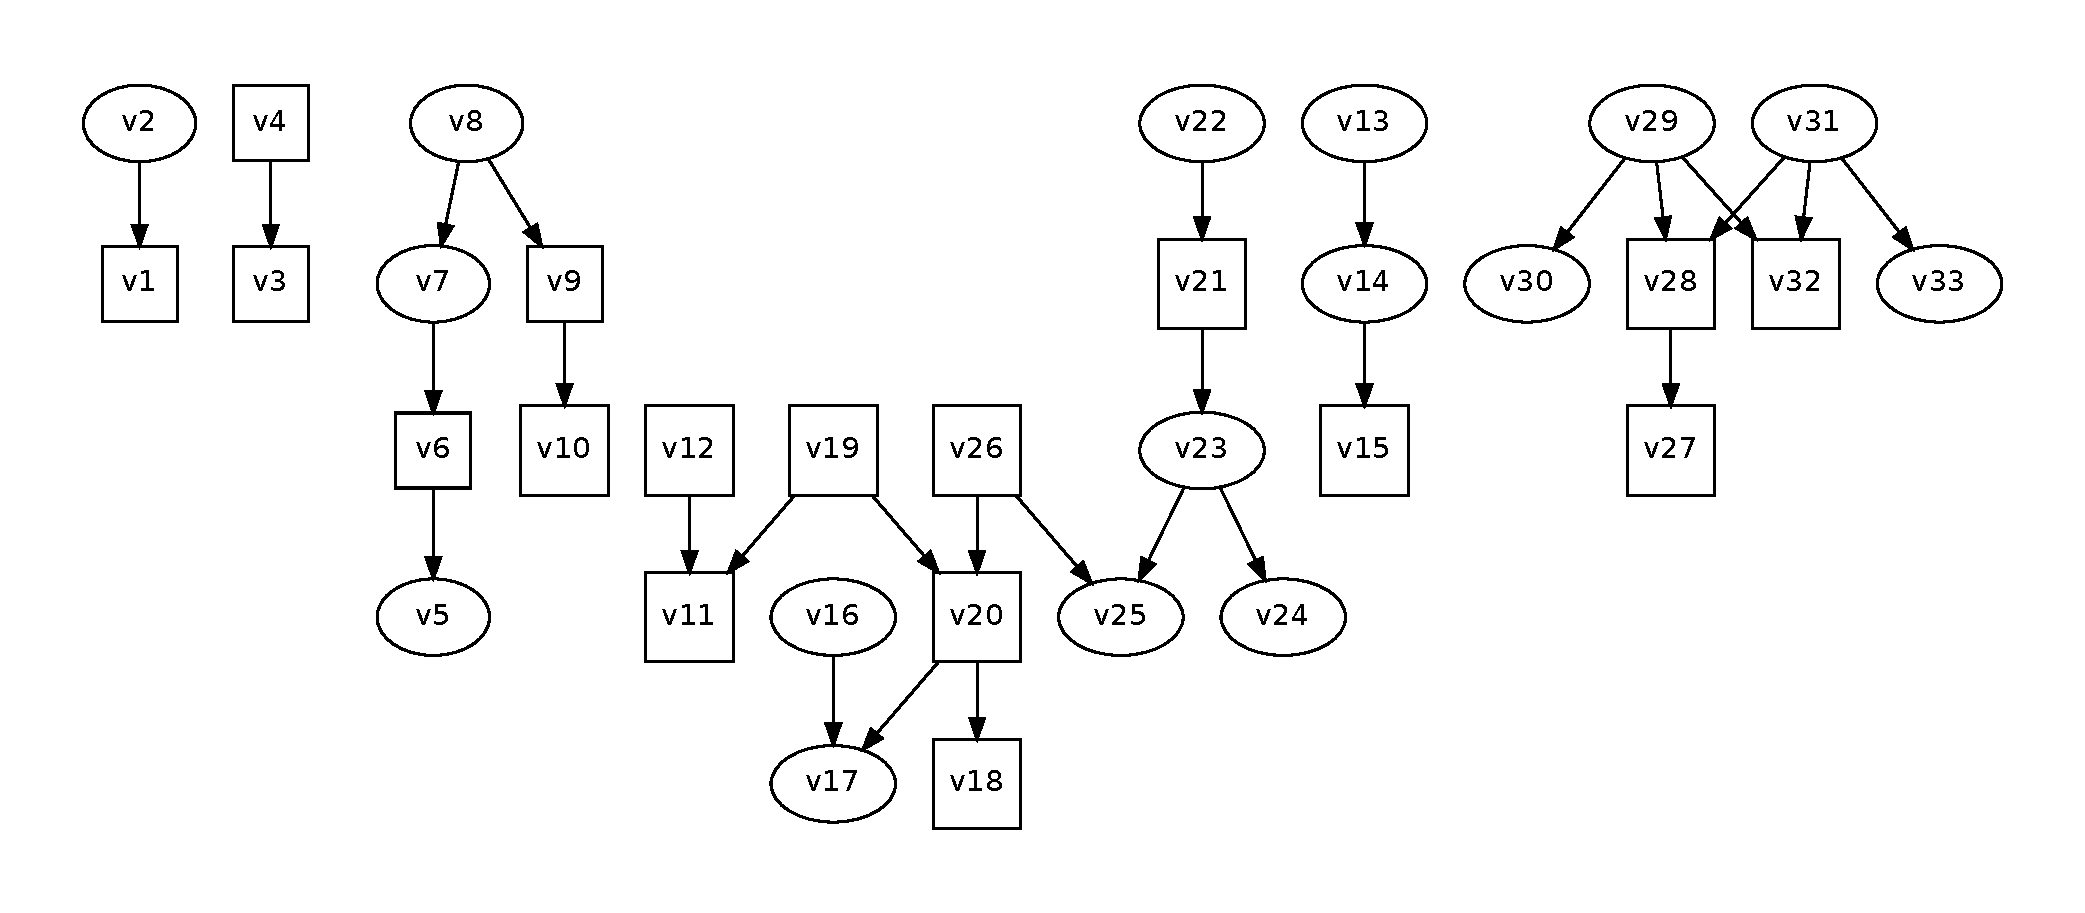
\includegraphics{dagcon}
\vspace{-1.0cm}
\caption{Example majority consensus network (from the results of only 10 searches)} \label{fig5}
\end{figure}


\begin{Schunk}
\begin{Sinput}
> # use results from above searches which are stored in ``myres''
> #step 1. discard any duplicate searches (these are unlikely)
> indexes<-uniquenets(myres$init.dag);
> all.res<-list();
> all.res$init.score<-myres$init.score[indexes];
> all.res$final.score<-myres$final.score[indexes];
> all.res$init.dag.<-myres$init.dag[indexes];
> all.res$final.dag<-myres$final.dag[indexes];
> # for every possible arc calculate how many times it appears in the searches  
> mypruneddags<-arcfreq(all.res$final.dag);
> # now get a matrix/DAG for the majority network comprising of 1/0s
> myfunc<-function(arg1,threshold,netdata){#trivial helper for apply()
+          if(arg1>=round(threshold*length(netdata$final.dag)))
+          {return(1);} else {return(0);}}
> dag.con<-apply(mypruneddags,c(1,2),FUN=myfunc,threshold=0.51,
+                netdata=all.res);
> tographviz(dag=dag.con,data.df=var33,outfile="dagcon.dot");#create file
> # dagcon.dot can then be processed with graphviz
> # unix shell "dot -Tpdf dagcon.dot -o dagcon.pdf" or use gedit if on Windows
> 
\end{Sinput}
\end{Schunk}


\section{Creating a Summary Network - Pruning}
Rather than use the majority consensus network as the most appropriate model of the data, an alternative approach is to choose the single best model found during a large number of searches. To determine sufficient heuristic searches have been run to provide reasonable coverage of all the features of the model landscape, then again checking for a stable majority consensus network as in Section \ref{mcn}, seems a sensible approach. Once the best overall DAG has been identified then the next task is to check this model for over-fitting. Unlike with the majority consensus network, which effective ``averages'' over many different competing models and therefore should generally comprise only robust structural features, choosing the DAG from a single model search is far more likely to contain some spurious features. When dealing with smaller data sets, say, of several hundred observations then this is extremely likely, as can easily be demonstrated using simulated data. A simple assessment of overfitting can be made by comparing the number of arcs in the majority consensus network with the number of arcs in the best fitting model. We have found that in larger data sets the majority consensus and best fitting model can be almost identical, while in smaller data sets the best fitting models may have many more arcs - suggesting a degree of overfitting. 

An advantage of choosing a DAG from an individual search is that unlike averaging over lots of different structures, as in the construction of a majority consensus network, the model chosen here has a structure which was actually found during a search across the model landscape. In contrast, the majority consensus network is a derived model which may never have been found chosen during even an exhaustive search, indeed it may even comprise of contradictory features as is a usual risk in averaging over different explanations (models) of data. In addition, a majority consensus network need also not be acyclic, although in practice this can be easily corrected by reversing one or more arcs to produce an appropriate DAG.

A simple compromise between the risk of over-fitting in choosing the single highest scoring DAG, and the risk of inappropriately averaging across different distinct data generating processes, is to prune the highest scoring DAG using the majority consensus model. In short, an element by element multiply of the highest scoring DAG and the majority consensus DAG, which gives a new DAG which only contains the structural features in \emph{both} models. 

\section{Creating a Summary Network - Parametric Bootstrapping}   
In \citeauthor{Friedman1999} (\citeyear{Friedman1999}) a general approach for using parametric bootstrapping to select BN models/DAG structures was presented. Such approaches can be reasonably easily implemented by using readily available Markov chain Monte Carlo sampling software such as JAGS or WinBUGS. The basic idea is to take the structure with the best network score and then code it up in either JAGS or WinBUGS, and use these samplers to generate bootstrap data sets from this model. That is, independent realisations from the model which can be used to generate a data set of the same size as the observed data. Given this bootstrap data, then the BN model search is repeated treating this as the observed data. By generating many bootstrap data sets and conducting searches on each, then this allows us to estimate the percentage support for each arc in the highest scoring model. Another way to put this is that we find out how many of the arcs in the highest scoring model can be ``recovered'' from a data set of the size as that actually observed. Obviously, the more data, the more statistical power, and the more structural features which can be recovered. For arcs with a lower level of support, e.g. <50\%, then these can be pruned from the best fitting model, the assumption being that these are potentially as a result of overfitting. The resulting model - possibly with arcs pruned off from the original model - is then our chosen model of the data. 

Using a 50\% threshold for arc support is intuitively reasonable as can be seen by considering a model of a single node. Suppose there are two covariates, and the ``response'' variable (the node) is almost deterministically dependent with each of these variables (that is overwhelming statistical support), and that the two covariates are almost exactly collinear. In which case only one arc will be needed in the model, and running random restart heuristic searches in this case will result in approximately 50\% of search results suggesting an arc from covariate one to the response variable, and the other 50\% for an arc from covariate two to the response variable. Therefore,  despite the fact that each of these variables is almost surely (with probability=1) dependent with the response variable each arc cannot exceed 50\% support. This is an idealized example but provides an intuitive argument as to why 50\% is a reasonable threshold above which we can be fairly confident that the arcs may be a real, rather than spurious statistical feature. 

While parametric bootstrapping is a general technique is well established and conceptually elegant, this may in practice not be computationally feasible. Even if taking the least demanding approach of conducting only one heuristic search per bootstrap data set, the number of data sets/searches required in order to get robust \% support values for each arc in the best fitting model may be large, and beyond what is reasonably possible even using high performance computing (HPC) hardware. We would suggest that it is at least good practice to investigate the feasibility of this approach. To that end we next outline how to perform parametric bootstrapping using {\tt abn} and {\tt JAGS} and all the relevant source files are included in the {\tt abn/bootstrapping\_example} library subdirectory.


\subsection{Steps Necessary to Perform Parametric Bootstrapping}
Given a BN model - DAG structure plus parameter priors - then the first step is to estimate the posterior parameters. The second step is to implement the DAG structure together with the posterior parameters into the language used by {\tt JAGS}, which is very similar to that used in {\tt WinBUGS}. Generally speaking, the posterior parameters in an additive BN model need not conform to any standard probability distribution as these are non-conjugate models. To make the implementation as general as possible, rather than, for example, attempting to match each posterior distribution to, say, the closest shaped Gaussian density, we present an approach which allows all posterior parameters to be from a non-standard - bespoke - distribution. This is implemented in {\tt JAGS} by discretising each posterior density across a fine grid and using a discrete sampler, {\tt dcat()} in {\tt JAGS}.   

\subsubsection{Estimating Posterior Densities}
The function {\tt getmarginal()} uses Laplace approximations to estimate the posterior density of each parameter in a BN model. An appropriate domain (range) for each parameter \emph{must} be supplied by the user which is done by some trial and error to find where about on the real line the density resides - it will be close to the origin either through the use of a logistic link function or through the standardisation of the Guassian node. An initial guess of (-2,2) is often a good starting point. It is crucially important that a sufficiently wide range is given so that ``all'' of the upper and lower tails of the distribution are included, e.g. the range should be where an R density plot first drops to approximately zero at each tail. Note that {\tt getmarginal()} works with one node and one parameter in that node at a time. It is not necessary - but does no harm - to specify the full DAG, but all that is needed is the node and its parents.  

We now follow the example contained in the {\tt abn/bootstrapping\_example} library subdirectory. We use a second data set included with {\tt abn}, called {\tt pigs.1par} which is again a synthetic dataset generated from analyses of real data. The first step is define the model of interest, {\tt mydag}, and then  estimate the posterior densities. The posterior parameters calculated are the marginal effects, that is all other model parameters (at the given node) are integrated out. At each node - which is defined using argument {\tt whichnode} - the intercept term can be estimated using {\tt whichvar=constant} (see below) and for Gaussian nodes the precision parameter can be estimated using {\tt whichvar=precision}. The remaining parameters are the mean covariate effects, for example using {\tt whichnode=D1} and {\tt whichvar=D2} in {\tt getmarginal()} gives the posterior marginal density for covariate {\tt D2} for the response variable {\tt D1}. Note that by default all Gaussian variables are standardised to a mean of zero and a standard deviation of one. 

\begin{Schunk}
\begin{Sinput}
> #specific a DAG model - the model we wish to use to perform 
> #parametric bootstrapping
> mydag<-matrix(c(
+ # D1 D2 D3 D4 D5 D6 D7 D8 D9 D10 Year Loc.x Loc.y
+   0, 1, 0, 0, 0, 0, 0, 0, 0, 0,  0,   0,    0,    # D1
+   0, 0, 1, 0, 0, 0, 0, 0, 0, 0,  0,   0,    0,    # D2
+   0, 0, 0, 1, 0, 0, 0, 0, 0, 0,  0,   0,    0,    # D3
+   0, 0, 0, 0, 0, 0, 0, 0, 0, 0,  0,   1,    0,    # D4
+   0, 0, 0, 0, 0, 1, 0, 0, 0, 0,  0,   0,    0,    # D5
+   0, 0, 0, 1, 0, 0, 0, 0, 0, 0,  0,   0,    0,    # D6
+   0, 0, 0, 0, 0, 0, 0, 0, 0, 0,  1,   0,    0,    # D7
+   0, 0, 0, 0, 0, 0, 0, 0, 0, 1,  0,   0,    0,    # D8
+   0, 1, 0, 0, 0, 0, 0, 0, 0, 0,  0,   0,    0,    # D9
+   0, 0, 0, 0, 0, 0, 0, 0, 1, 0,  0,   0,    0,    # D10
+   0, 0, 0, 0, 0, 0, 0, 0, 0, 0,  0,   0,    0,    # Year
+   0, 0, 0, 0, 0, 0, 1, 0, 0, 0,  0,   0,    0,    # Loc.x
+   0, 0, 0, 0, 0, 0, 1, 0, 0, 0,  0,   0,    0     # Loc.y
+                                                ),byrow=TRUE,ncol=13); 
> colnames(mydag)<-rownames(mydag)<-names(pigs.1par);#set names
> 
\end{Sinput}
\end{Schunk}
\begin{Schunk}
\begin{Sinput}
> # Node D1|D2 e.g. logit(P(D1=TRUE)=constant+coeff*D2
> # first get the posterior density for the constant
> marg<-getmarginal(data.df=pigs.1par,
+                    dag.m=mydag,
+                    whichnode="D1",
+                    whichvar="constant",#this is the intercept
+                      post.x=seq(from=1,to=1.7,len=1000),
+                      verbose=FALSE,std=TRUE);
> # get grid of discrete values x and f(x)
> D1.p<-cbind(marg[,1],marg[,2]);
> # now repeat for the slope term coeff
> marg<-getmarginal(data.df=pigs.1par,
+                    dag.m=mydag,
+                    whichnode="D1",
+                    whichvar="D2",#this is the slope
+                      post.x=seq(from=0.6,to=1.5,len=1000),
+                      verbose=FALSE,std=TRUE);
> # add to existing grid x,f(x),x,f(x)
> D1.p<-cbind(D1.p,marg[,1],marg[,2]);
\end{Sinput}
\end{Schunk}

Figure \ref{fig6}
\begin{figure}[htbp]
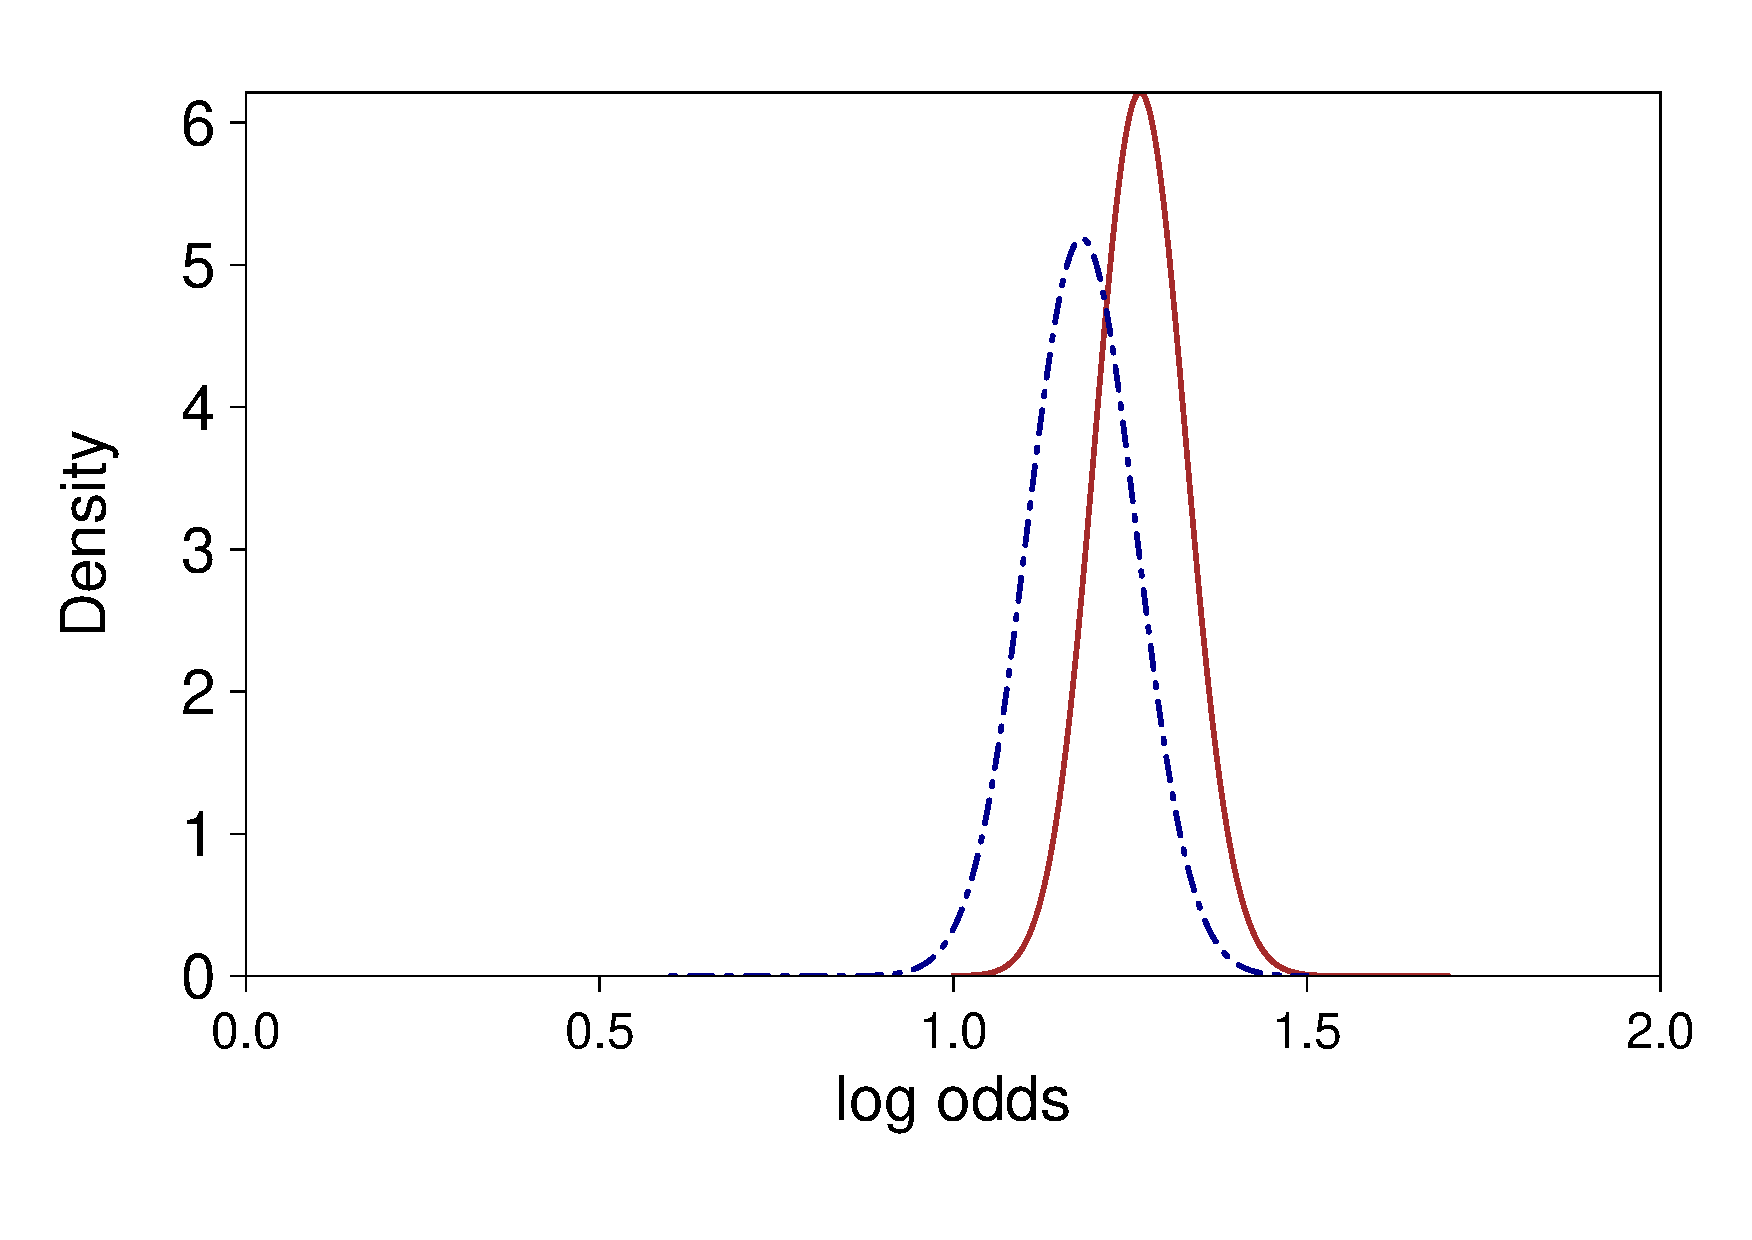
\includegraphics{abn-017}
\caption{Posterior densities for intercept and slope in node D1 in pigs.1par} \label{fig6}
\end{figure}
shows an example of posterior densities estimated using {\tt getmarginal()}, all posterior densities for all parameters in the additive BN can be estimated in the same way.

The file {\tt calculate\_marginalDensities.R} in {\tt abn/bootstrapping\_example} contains R code for estimating all the marginal parameters in the DAG {\tt mydag} given above. This file is documented. It calculates all the marginal distributions and then writes them out to a file {\tt post\_params.R} which is in the R dump format which can be read into {JAGS}.

The remaining files are {\tt script1.R} which is the script which runs the {\tt JAGS} MCMC sampling. The {\tt JAGS} package is open source and can be downloaded from sourceforge along with appropriate documentation. The file {\tt simulate\_1par.bug} contains the DAG implemented into the {\tt JAGS} language along with the posterior parameter estimates, the creation of this file is the main task involved in the parameteric bootstrapping. Once the {\tt script1.R} has completed (this script is run simply by typing {\tt jags script1.R} at the command line), then the bootstrap data set generated is contained in the file {\tt outchain1.txt} and {\tt outchain2.txt}. Running two (or more) chains allows for checking of convergence. The script is set up to generate 10000 realisations, to get a single bootstrap data set we would trim this down to 9011 observations which is that same size as the original data {\tt pigs.1par}. Once we have this bootstrap data set then we simply run a model search on this, for example using {\tt hillsearchabn()} as detailed above.  

To automate the parametric bootstrapping one option is to edit the {\tt script1.R} so that sufficient realisations are generated to create many independent bootstrap data sets, for example generate 1000 $\times$ 9011 realisations. It is straightforward to edit the above {\tt hillsearchabn()}, for example by putting the call to {\tt hillsearchabn()} inside a loop which iterates through different bootstrap data sets. Note that it is far more efficient to call {\tt hillsearchabn()} once inside each iteration than use {\tt searchabn()}, as the latter is designed to provide indepth output at individual search level and may be over twice as slow as calling {\tt hillsearchab()} using {\tt num.searches=1}.    

\section{Order Based Searches}
It is generally not feasible to iterate over all possible DAG structures when dealing with more than a handful of variables, hence the reliance on heuristic searches. It is also extremely difficult to construct efficient Monte Carlo Markov chain samplers across BN structures. A solution to this was proposed in \citeauthor{Friedman2003} (\citeyear{Friedman2003}) where rather than sample across DAGs, it was proposed to sample across node orderings. A node order is simply the set of integers $1$ through $n$, where $n$ is the number of variables in the data. A DAG is consistent with an ordering if for each node in the order its parents come before it. For example a DAG with only an arc from 1$\rightarrow$2 is consistent with ordering $1,2,3,4$ as the parent $1$ comes before $2$, but a DAG with an arc from 2$\rightarrow$1 is not consistent with this ordering. In effect, each order is a collection of DAGs, and note that each DAG may be consistent with multiple orders, i.e. the empty DAG is consistent with every possible ordering. This introduces bias, in that a search across orders need not give the same results as a search across DAGs, if the latter were possible. This bias is towards more parsimonious models. The big advantage of searching across orders is that there are $n!$ different orders compared to at least $2^{ n \choose 2 }$ different DAGs.  

There are (at least) two approaches for searching across orders. The first is to construct a Markov chain which samples from the posterior distribution of all orders, and is the approach presented in \citeauthor{Friedman2003} (\citeyear{Friedman2003}). Alternatively, in \citeauthor{Koivisto2004} (\citeyear{Koivisto2004}) an exact method is proposed which rather than sample across orders, performs an exhaustive search. This has the advantage that it can also be used to find the globally optimal DAG of the data - the most probable structure - as well as posterior probabilities for structural features, such as individual arcs. The drawback is that this exact approach is only feasible with smaller number of variables e.g. up to 12 or 13 when dealing with additive models. 

The {\tt abn} library has an implementation of the method due to \citeauthor{Koivisto2004} (\citeyear{Koivisto2004}) which allows for the computation of posterior probabilities for individual structural features, such as each arc, as well as the most probable structure. One potentially important point of note is that these posterior probabilities require the summing of probabilities across different structures and as such may be susceptible to numerical underflow errors (as it is not possible to perform this operation on a log scale) for data sets with larger numbers of observations. This does not apply to finding the most probable structure as this involves maximisation which can be done on a log scale. 

\subsection{Exact Posterior Probabilities of Structural Features}
We now demonstrate how to determine posterior probabilities for individual structural features using a small subset of observations and 10 variables from the {\tt pigs.1par} data. This uses the {\tt allnodesabn()} and {\tt getposteriorfeaturesbn()} functions. There is also an equivalent for conjugate multinomial BN models {\tt allnodesabn()}. The same function, {\tt getposteriorfeaturesbn()}, works for both conjugate and additive models as it only involves the DAG and not the parameterisation. Only a small number of observations are used here to avoid numerical underflow problems. In some data sets underflow may not be a problem, as this is very much a data specific issue. In any case your mileage may vary.

\begin{Schunk}
\begin{Sinput}
> pigs<-pigs.1par[1:50,c(2,3)];#take a subset of observations and variables
> ## step 1. find all the local scores within each node - this creates a "cache"
> ## of scores
> ## n.b. using a parent limit of 1 e.g we only consider DAGs with at most one 
> ## arc per node
> mynodes.add<-allnodesabn(data.df=pigs,max.parents=1); 
\end{Sinput}
\begin{Soutput}
processing node...1
processing node...2
\end{Soutput}
\begin{Sinput}
> ## step 2. search across all orders/DAGs for the given structural feature
> # specifically calculate the get posterior prob of arc 1->2 
> p.2.1<-getposteriorfeaturesbn(local.scores=mynodes.add,feature="arc",child=2,
+                               parent=1);
> print(p.2.1);
\end{Sinput}
\begin{Soutput}
[1] 3.980759e-29
\end{Soutput}
\begin{Sinput}
> #now for arc 2->1
> p.1.2<-getposteriorfeaturesbn(local.scores=mynodes.add,feature="arc",child=1,
+                               parent=2);
> print(p.1.2);
\end{Sinput}
\begin{Soutput}
[1] 3.983062e-29
\end{Soutput}
\begin{Sinput}
> ## step 3. calculate the denominator - across all structural features (see text)
> denom<-getposteriorfeaturesbn(local.scores=mynodes.add,feature="all");
> print(denom);
\end{Sinput}
\begin{Soutput}
[1] 1.696262e-27
\end{Soutput}
\begin{Sinput}
> ## we now get the posterior probability for arc 1->2
> print(p.2.1/denom);
\end{Sinput}
\begin{Soutput}
[1] 0.02346783
\end{Soutput}
\begin{Sinput}
> ## we now get the posterior probability for arc 2->1
> print(p.1.2/denom);
\end{Sinput}
\begin{Soutput}
[1] 0.02348141
\end{Soutput}
\end{Schunk}

The posterior probability for each arc is calculated by marginalising over all possible other combinations. That is, it is the sum of the marginal likelihoods across all DAGs (analysed in blocks of orders) which contain this specific arc. The denominator here is the sum of marginal likelihoods across all DAGs (analysed in blocks of orders). Note that the very small numerical difference between these probabilities may be due to the fact that the additive model priors are not likelihood equivalent.

It is also possible to calculate the posterior probability for an arbitrary structural feature by specifying this in the call to {\tt getposteriorfeaturesbn()}. To illustrate this we use the simplest example of a two node network but this works in an analogous fashion for larger numbers of variables.   

\begin{Schunk}
\begin{Sinput}
> pigs<-pigs.1par[1:50,c(2,3)];#simple 2 node model
> ## step 1. find all the local scores within each node - this creates a "cache"
> ##                                                                   of scores
> mynodes.add<-allnodesabn(data.df=pigs,max.parents=1); 
\end{Sinput}
\begin{Soutput}
processing node...1
processing node...2
\end{Soutput}
\begin{Sinput}
> print(mynodes.add);
\end{Sinput}
\begin{Soutput}
$node
[1] 1 1 2 2

$parents
     [,1] [,2]
[1,]    0    0
[2,]    0    1
[3,]    0    0
[4,]    1    0

$nodescore
[1] -26.39145 -29.40176 -35.99116 -39.00205

$restricted.parents
[1] 0
\end{Soutput}
\begin{Sinput}
> # now want the posterior prob. of the independence DAG (empty network)
> G<-c(1,0,1,0);#empty [1][2] - this says include rows 1 and 3 in the node cache
> # row 1 corresponds to node 1 having no parents and row 3 for node 2
> # with no parents
> DAG1<-getposteriorfeaturesbn(local.scores=mynodes.add,feature="custom",
+                              featuredefn=G);
> #now for DAG node 2 indep, node 1 depends on node 2
> G<-c(0,1,1,0);# [1|2][2]
> DAG2<-getposteriorfeaturesbn(local.scores=mynodes.add,feature="custom",
+                              featuredefn=G);
> #now for DAG node 1 indep, node 2 depends on node 1
> G<-c(1,0,0,1);# [1][2|1]
> DAG3<-getposteriorfeaturesbn(local.scores=mynodes.add,feature="custom",
+                              featuredefn=G);
> print(DAG1+DAG2+DAG3);#get total sum
\end{Sinput}
\begin{Soutput}
[1] 1.696262e-27
\end{Soutput}
\begin{Sinput}
> #this equals the denominator - which it should since this is all 
> #possible DAGs
> denom<-getposteriorfeaturesbn(local.scores=mynodes.add,feature="all",
+        child=NULL,
+        parent=NULL);
> print(denom);
\end{Sinput}
\begin{Soutput}
[1] 1.696262e-27
\end{Soutput}
\begin{Sinput}
> # posterior probabilities for the 3 DAGs, [1][2], [1|2][2],[2|1][1] are
> print(p1<-DAG1/denom);
\end{Sinput}
\begin{Soutput}
[1] 0.9530508
\end{Soutput}
\begin{Sinput}
> print(p2<-DAG2/denom);
\end{Sinput}
\begin{Soutput}
[1] 0.02348141
\end{Soutput}
\begin{Sinput}
> print(p3<-DAG3/denom);
\end{Sinput}
\begin{Soutput}
[1] 0.02346783
\end{Soutput}
\begin{Sinput}
> print(p1+p2+p3);
\end{Sinput}
\begin{Soutput}
[1] 1
\end{Soutput}
\end{Schunk}

Finally, as an aside it is possible to calculate the posterior probabilities for individual arcs also by also specifying a custom structure using argument {\tt featuredefn}. This shows explicitly how the marginalisation is done.
\begin{Schunk}
\begin{Sinput}
> pigs<-pigs.1par[1:50,c(2,3)];#simple 2 node model
> ## step 1. find all the local scores within each node - this creates a "cache"
> ##                                                                   of scores
> mynodes.add<-allnodesabn(data.df=pigs,max.parents=1); 
\end{Sinput}
\begin{Soutput}
processing node...1
processing node...2
\end{Soutput}
\begin{Sinput}
> print(mynodes.add);
\end{Sinput}
\begin{Soutput}
$node
[1] 1 1 2 2

$parents
     [,1] [,2]
[1,]    0    0
[2,]    0    1
[3,]    0    0
[4,]    1    0

$nodescore
[1] -26.39145 -29.40176 -35.99116 -39.00205

$restricted.parents
[1] 0
\end{Soutput}
\begin{Sinput}
> #arc 1->2, dont care about node 1 e.g. arc is marginalised over all possible
> #                                                         other combinations
> G<-c(1,1,0,1);
> p.2.1.G<-getposteriorfeaturesbn(local.scores=mynodes.add,feature="custom",
+                                 featuredefn=G);
> #arc 2->1, dont care about node 2
> G<-c(0,1,1,1);
> p.1.2.G<-getposteriorfeaturesbn(local.scores=mynodes.add,feature="custom",
+                                 featuredefn=G);
> # now get denominator 
> G<-c(1,1,1,1);
> denom<-getposteriorfeaturesbn(local.scores=mynodes.add,feature="custom",
+                                 featuredefn=G);
> print(p.2.1.G/denom);#post. prob. arc 1->2
\end{Sinput}
\begin{Soutput}
[1] 0.02346783
\end{Soutput}
\begin{Sinput}
> print(p.2.1/denom);  # as calculated directly above
\end{Sinput}
\begin{Soutput}
[1] 0.02346783
\end{Soutput}
\begin{Sinput}
> print(p.1.2.G/denom);#post. prob. arc 2->1
\end{Sinput}
\begin{Soutput}
[1] 0.02348141
\end{Soutput}
\begin{Sinput}
> print(p.1.2/denom);  # as calculated directly above
\end{Sinput}
\begin{Soutput}
[1] 0.02348141
\end{Soutput}
\end{Schunk}

To calculate arc $1\rightarrow2$ we simply set the value of {\tt featuredefn} so that every possible parent combination is included in every node in the network other than the child node, in this case node 2. In the child node we include all parent combinations which include arc $1\rightarrow2$. Note that iterating over orders also removes any cycles and all we need be concerned with is individual nodes and not how these fit together into a DAG.   

\subsection{Most Probable Structure}
Using the exact order based method due to \citeauthor{Koivisto2004} (\citeyear{Koivisto2004}) it is also possible to identify the DAG with globally best network score - subject to the bias present due to using an ordered based grouping of DAGs. Unlike calculating posterior probabilities of individual structural features, finding the most probable structure does not require the summing marginal likelihoods, but rather maximisation. Numerical underflow is therefore not a problem here, however, finding the most probably structure may not be computationally feasible for more than 12 or 13 nodes, at least when dealing with additive models which require considerably more numerical computational per DAG.

To calculate the most probable structure we again use {\tt allnodesabn()} to calculate a cache of individual node scores. Next, the function {\tt findmostprobablebn} does the actual exhaustive order based search, and works for both conjugate and additive models since as with calculating the posterior probabilities this step only involves structural searching and is not concerned with the precise parameterisation of each BN model.  

\begin{Schunk}
\begin{Sinput}
> pigs<-pigs.1par[,c(1:8,12,13)];#all 9011 observation but limit to 10 variables
> # using all 13 variables in pigs will take several hours of cpu time
> mynodes.add<-allnodesabn(data.df=pigs,max.parents=1); 
\end{Sinput}
\begin{Soutput}
processing node...1
processing node...2
processing node...3
processing node...4
processing node...5
processing node...6
processing node...7
processing node...8
processing node...9
processing node...10
\end{Soutput}
\begin{Sinput}
> ## now for most probable network of all DAGs where each node has at
> ## most one arc
> map.1par.10var<-findmostprobablebn(local.scores=mynodes.add,data.df=pigs);
> tographviz(dag=map.1par.10var,data.df=pigs,outfile="map1_10var.dot");#create file
> # mydag.dot can then be processed with graphviz
> # unix shell "dot -Tpdf map1_10var.dot -o map1_10var.pdf" or use gedit if on Windows
\end{Sinput}
\end{Schunk}

Figure \ref{fig7}
\begin{figure}[htb]\hspace{4.0cm}
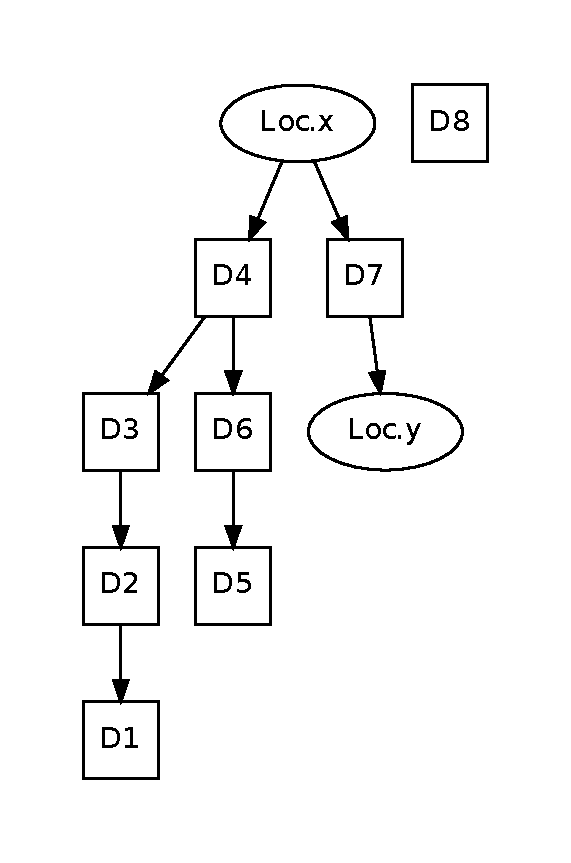
\includegraphics[angle=0,scale=0.5]{map1_10var}
\caption{Most probable DAG for data in pigs.1par with variables D1-D8, Loc.x and Loc.y, and after imposing a limit of no more than one parent per node} \label{fig7}
\end{figure}
shows a most probable DAG using a subset of variables from pigs.1par and a parent limit of one per node. 

\begin{Schunk}
\begin{Sinput}
> pigs<-pigs.1par;#all observations all variables
> mynodes.add<-allnodesabn(data.df=pigs,max.parents=1); 
> ## now for most probable network of all DAGs where each node has at
> ## most one arc
> system.time(map.1par<-findmostprobablebn(local.scores=mynodes.add,data.df=pigs));
> tographviz(dag=map.1par,data.df=pigs,outfile="map_1par.dot");#create file
> # mydag.dot can then be processed with graphviz
> # unix shell "dot -Tpdf map_1par.dot -o map_1par.pdf" or use gedit if on Windows
\end{Sinput}
\end{Schunk}
\clearpage
Figure \ref{fig8}
\begin{figure}[htb]\hspace{4.0cm}
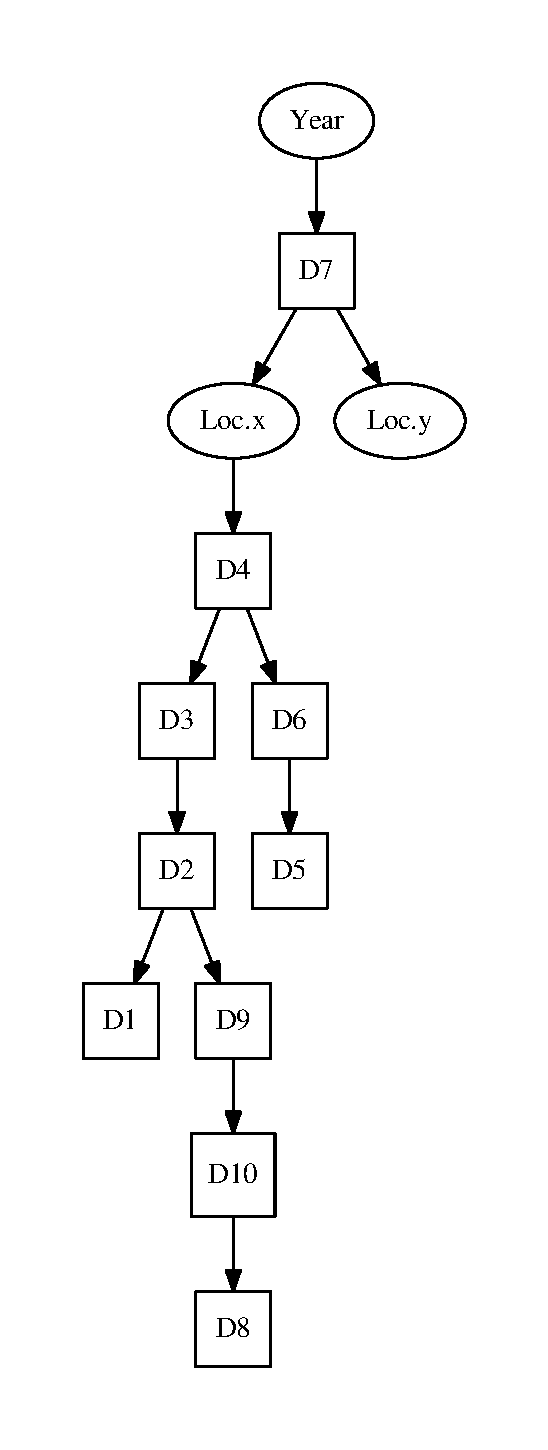
\includegraphics[angle=0,scale=0.5]{map_1par}
\caption{Most probable DAG for data in pigs.1par imposing a limit of no more than one parent per node} \label{fig8}
\end{figure}
shows the most probable DAG considering all variables in pigs.1par and a parent limit of one per node. This took 6520 seconds ($\approx$1.8 hrs) to complete on an 3Ghz Intel Xeon CPU, and the runtime may increase dramatically for more variables and an increased parent limit.
\clearpage
\section{Summary}
The {\tt abn} library provides a range of Bayesian network models to assist with identifying statistical dependencies in complex data, in particular models which are multidimensional analogues of generalised linear models. This process is typically referred to as structure learning, or structure discovery, and is computational extremely challenging. Heuristics are the only options for data comprising of larger numbers of variables. As with all model selection, over-modelling is an everpresent danger and using either: i) summary models comprising of structural features present in many locally optimal models or else; ii) using parametric bootstrapping to determine the robustness of the features in a single locally optimal model are likely essential to provide robust results. An alternative presented was exact order based searches, in particular finding the globally most probable structure. This approach is appealing as it is exact, but despite collapsing DAGs into orderings for larger scale problems it may not be feasible.   

\newpage
\bibliography{abn}

\end{document}
